\documentclass[sigconf,numbers,sort&compress,colorlinks]{acmart}

\usepackage{booktabs} % For formal tables
\usepackage{acro}
\usepackage{listings}
\usepackage{hyperref}
\usepackage{graphicx}
\usepackage{caption}
\usepackage{amsmath, amssymb, graphics, setspace}

\usepackage[nameinlink]{cleveref}
\crefformat{figure}{#2(fig. #1)#3}
\Crefformat{figure}{#2(Fig. #1)#3}
\crefrangeformat{figure}{#3(fig. #1#4 to #5#2)#6}
\Crefrangeformat{Figure}{#3(fig. #1#4 to #5#2)#6}

% Make citations use ieee format
\setcitestyle{square,citesep={], [}}
\makeatletter
\def\NAT@def@citea{\def\@citea{\NAT@separator}}
\makeatother

\graphicspath{ {pictures/} }

% Copyright
%\setcopyright{none}
%\setcopyright{acmcopyright}
%\setcopyright{acmlicensed}
\setcopyright{rightsretained}
%\setcopyright{usgov}
%\setcopyright{usgovmixed}
%\setcopyright{cagov}
%\setcopyright{cagovmixed}


% DOI
\acmDOI{10.475/123_4}

% ISBN
\acmISBN{123-4567-24-567/08/06}

%Conference
\acmConference[AMP Lab '18]{ACM Autonomous Mastery Prototyping Lab conference}{November 2018}{Blacksburg, Virgina, USA}
\acmYear{2018}
\copyrightyear{2018}

\DeclareAcronym{iot}{
    short = IoT,
    long = Internet of Things,
    class = acron
}
\DeclareAcronym{rfid}{
    short = RFID,
    long = Radio Frequency Identification,
    class = acron
}
\DeclareAcronym{usn}{
    short = USN,
    long = Ubiquitous Sensor Network,
    class = acron
}
\DeclareAcronym{rfi}{
    short = RFI,
    long = Radio Frequency Interference,
    class = acron
}
\DeclareAcronym{emi}{
    short = EMI,
    long = Electromagnetic Interference,
    class = acron
}
\DeclareAcronym{dc}{
    short = DC,
    long = Direct Current,
    class = acron
}
\DeclareAcronym{ac}{
    short = AC,
    long = Alternating Current,
    class = acron
}
\DeclareAcronym{cdf}{
    short = CDF,
    long = Cumulative Distribution Function,
    class = acron
}

\begin{document}

\title{\ac{iot} Hardware Security: Exploring Thermocouple Vulnerabilities}

\author{Ryan Burrow}
\affiliation{Virginia Tech}
\email{rsardb11@vt.edu}

\author{Steven Frederiksen}
\affiliation{Virginia Tech}
\email{sfrederiksen@vt.edu}

\author{Daulet Talapkaliyev}
\affiliation{Virginia Tech}
\email{kosovo@vt.edu}


\begin{abstract}
This paper explores attacks on \ac{iot} devices through exploitation of the physics of the sensors that they rely on. We implemented a simple thermocouple interference experiment demonstrating how a thermocouple could be interfered with remotely. As a solution to this problem, we implemented a software-based controller that can detect interference and replace the faulty data with a steady-state model of the thermocouple.
\end{abstract}

%
% The code below should be generated by the tool at
% http://dl.acm.org/ccs.cfm
% Please copy and paste the code instead of the example below.
%
\begin{CCSXML}
<ccs2012>
<concept>
<concept_id>10002978.10002979.10002983</concept_id>
<concept_desc>Security and privacy~Cryptanalysis and other attacks</concept_desc>
<concept_significance>500</concept_significance>
</concept>
<concept>
<concept_id>10002978.10002997.10002999</concept_id>
<concept_desc>Security and privacy~Intrusion detection systems</concept_desc>
<concept_significance>500</concept_significance>
</concept>
<concept>
<concept_id>10002978.10003001.10003002</concept_id>
<concept_desc>Security and privacy~Tamper-proof and tamper-resistant designs</concept_desc>
<concept_significance>500</concept_significance>
</concept>
</ccs2012>
\end{CCSXML}

\ccsdesc[500]{Security and privacy~Cryptanalysis and other attacks}
\ccsdesc[500]{Security and privacy~Intrusion detection systems}
\ccsdesc[500]{Security and privacy~Tamper-proof and tamper-resistant designs}

\keywords{Cybersecurity, Embedded Systems, \ac{iot}, Thermocouples}

\maketitle

\section{Introduction}

\subsection{\ac{iot} Security}

The ability of ``things'' to connect and interact with each other over the Internet with minimum human involvement makes Internet of Things a new step in technological progress. Thanks to the widespread use of wireless technology and the emergence of cloud computing, the \ac{iot} is growing at an astronomical pace and is expected to reach ``more than 20 billion internet connected things by 2020'' \cite{Gartner17}. However, while \ac{iot} ecosystem can greatly benefit our life, uncontrollable growth of internet-connected devices leads to increased security and privacy risks. Heterogeneous nature of \ac{iot} systems, which can combine millions of distinctive devices, infrastructures and applications, makes it extremely difficult to develop uniform security standards and policies. This greatly widens the attack surface of \ac{iot} devices and makes them particularly attractive to hackers. 

To discuss cybersecurity of any system, we must understand its architecture. Three-layer model is one of the most commonly used \ac{iot} architecture models. The three comprehensive layers/levels in this model are: perception layer, network layer and application layer \cite{Mendez17,Deogirikar17,Krishna17}. Perception layer is responsible for reliable collection of data from various sensors. Perception layer is often built using \ac{rfid} tags and \acp{usn}, which help identify objects and obtain any necessary environmental information \cite{Devera14,Deng12}. Network layer must provide ubiquitous access and reliably transfer any data collected at perception layer. Network layers primarily use wireless communication standards like ZigBee, BLE, Bluetooth (WPAN) and WiFi (WLAN). Application layer is any information processing system that stores and analyzes the received information to appropriately manage an application or a service \cite{Yang17}. In context of cybersecurity each layer can be viewed as separate attack surface with unique vulnerabilities and exploits. Moreover, the interconnectedness of \ac{iot} devices at each layer means that every insufficiently protected device connected to the network can affect the overall level of safety and sustainability of the whole \ac{iot} system. This paper mainly focuses on the perception layer and physical attacks, as we propose a transduction attack on K-type thermocouple sensors and a possible software-based countermeasure. 

\subsection{Thermocouple sensors}

\begin{figure}
    \centering
    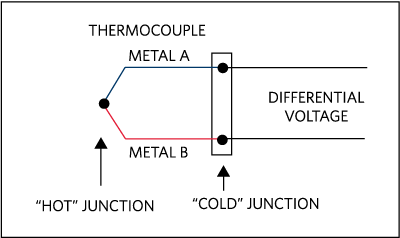
\includegraphics[width=\linewidth]{pictures/TC.png}
    \caption{Fundamental thermocouple \cite{Ismail17}}
    \label{fig:TCouple}
\end{figure}

Thermocouple is an electric device that utilizes Seebeck effect to measure temperatures at the junction of two dissimilar metals/wires (\cref{fig:Thermocouple}). No power consumption, cost-effectiveness and reasonable accuracy makes K-type thermocouples industry-standard temperature-measuring method \cite{Duff10}. Unfortunately, due to microvolt-level signal changes (~40$\mu$V/\textdegree{}C in K-type), thermocouples are quite susceptible to \ac{emi}/\ac{rfi} \cite{Smalcerz2013,Astm93}. \ac{emi} in this case is any undesirable effects of electromagnetic, electric and magnetic fields, which can degrade the quality of the system due to distortion of the useful signal \cite{Getz96}. This means that without proper physical protection or signal filtering (analog and/or digital) such sensors can be vulnerable to stray noise or a range of intended physical attacks. While proper shielding and dedicated filters can greatly reduce such interference, they can also make an otherwise cheap and robust sensors quite costly and complex. 

To test the susceptibility of thermocouple sensors to electromagnetic vulnerabilities, we experimented with one of the possible physical attacks - inducing voltage in the thermocouple wires. Generally, there are two ways in which electromagnetic fields can significantly skew the thermocouple readings: ``induction heating of the thermoelements and induced voltage in the thermocouple wires'' \cite{Omega17}. Heat induction happens at very high amplitudes or high frequencies, when induced currents from alternating magnetic field heat the thermoelement itself, thus affecting the measurement readings. Inducing voltage in thermocouple wires on the other hand, does not require a large field to make any alteration to the temperature output. Since thermocouples measure microvolt-level signal changes, inducing even a small voltage in thermocouple wires can affect the accuracy of the readings. Electromagnetic induction in this case can be explained using Faraday's law of induction \cref{fig:Thermocouple}, which states that ``induced electromotive force (i.e. voltage) in any closed circuit is equal to the rate of change of the magnetic flux enclosed by the circuit'' \cite{Jordan68}. 

\begin{equation}
\begin{split}
\varepsilon = - N\frac{\mathrm{d\Phi _{B}} }{\mathrm{d} t},
\end{split}
\qquad
\begin{split}
\varepsilon - Electromotive force\\
{\Phi _{B}} - magnetic flux\\
N - number of coil turns
\end{split}
\end{equation}

\begin{figure}
    \centering
    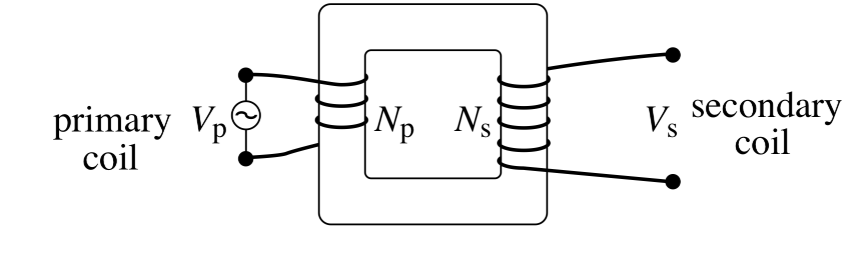
\includegraphics[width=\linewidth]{pictures/FLaw.png}
    \caption{Basic transformer (function by applying Faraday’s law of induction) \cite{Flap96}}
    \label{fig:Transformer}
\end{figure}


Inducing large voltages can allow the adversary to not only introduce electromagnetic noise to the thermocouple sensors, but completely manipulate the temperature readings. Given a reasonably large amplitude/frequency, the attacker can skew the temperature outputs from thermocouple towards impossibly low or high values [11]. Depending on the final application, incorrect readings from such thermocouple sensors can result in minor inconvenience (home thermostats) or in major accident (flame sensors in gas appliances). 

There are few common solutions to general \ac{emi}/\ac{rfi} problem, like \ac{rfi} filters, differential-input amplifiers, low-pass filters, etc. \cite{Duff10}. However, when the attack is highly directional and operates at high amplitude/frequency, these solutions can make thermocouple systems very expensive and complex. Alternative methods would be software-based countermeasures that focus on anomaly detection algorithms and an appropriate response \cite{Amitai16}. In this paper we propose a software-based countermeasure, which includes a simple guard logic and alert/response algorithm, to help the \ac{iot} sensor systems detect and thwart common transduction attacks.

This paper is organized as follows. In \cref{hwi}, we describe in detail our experiment with one of the transduction attacks on K-type thermocouples. \cref{swi} focuses on our signal filter application, which was implemented in software and can potentially help thwart such attacks. \cref{disc} includes a discussion and analysis of our experiment and simulation results. In \cref{fut}, we look at the possible next steps for this project, such as alternative transduction attacks and some potential improvements to our countermeasure implementation. A brief conclusion is given in \cref{conc}.



%\subsubsection{Privacy}

%\subsubsection{Hardware related issues}

% Types of issues



% Examples



%\subsection{Proposed Method}

%\subsubsection{Interference}

% EM



% RF



% Induction



% Equations



%\subsubsection{Software}

% Model



% Guard Logic



% Response

\section{Hardware Implementation}\label{hwi}
\subsection{What we did}\label{wwd}
As described in the introduction, we focused on replicating the interference shown in \cite{Fu18} through electromagnetic coupling between an emitter and a thermocouple. The equipment used was as follows: RIGOL DG4162 Function Generator \cref{fig:FGen}, 30-turn copper inductor (\cref{fig:Inductor}), 6-in Type-K thermocouple \cref{fig:Thermocouple}, MAX31856 thermocouple breakout board \cref{fig:MAX31856}, and a Tektronix DPO 3034 oscilloscope on the thermocouple outputs \cref{fig:DPO3034}. No modifications were performed on the equipment. The basic setup for our experiments is shown in \cref{fig:Block}.

% % Here is how to insert a picture
% \begin{figure}
% \label{this-is-my-label}
% \includegraphics{fly}
% \caption{A sample black and white graphic.}
% \end{figure}
\begin{figure}
    \centering
    \includegraphics[width=\linewidth]{Function-Gen-Pic.jpg}
    \caption{RIGOL DG4162}
    \label{fig:FGen}
\end{figure}
\begin{figure}
    \centering
    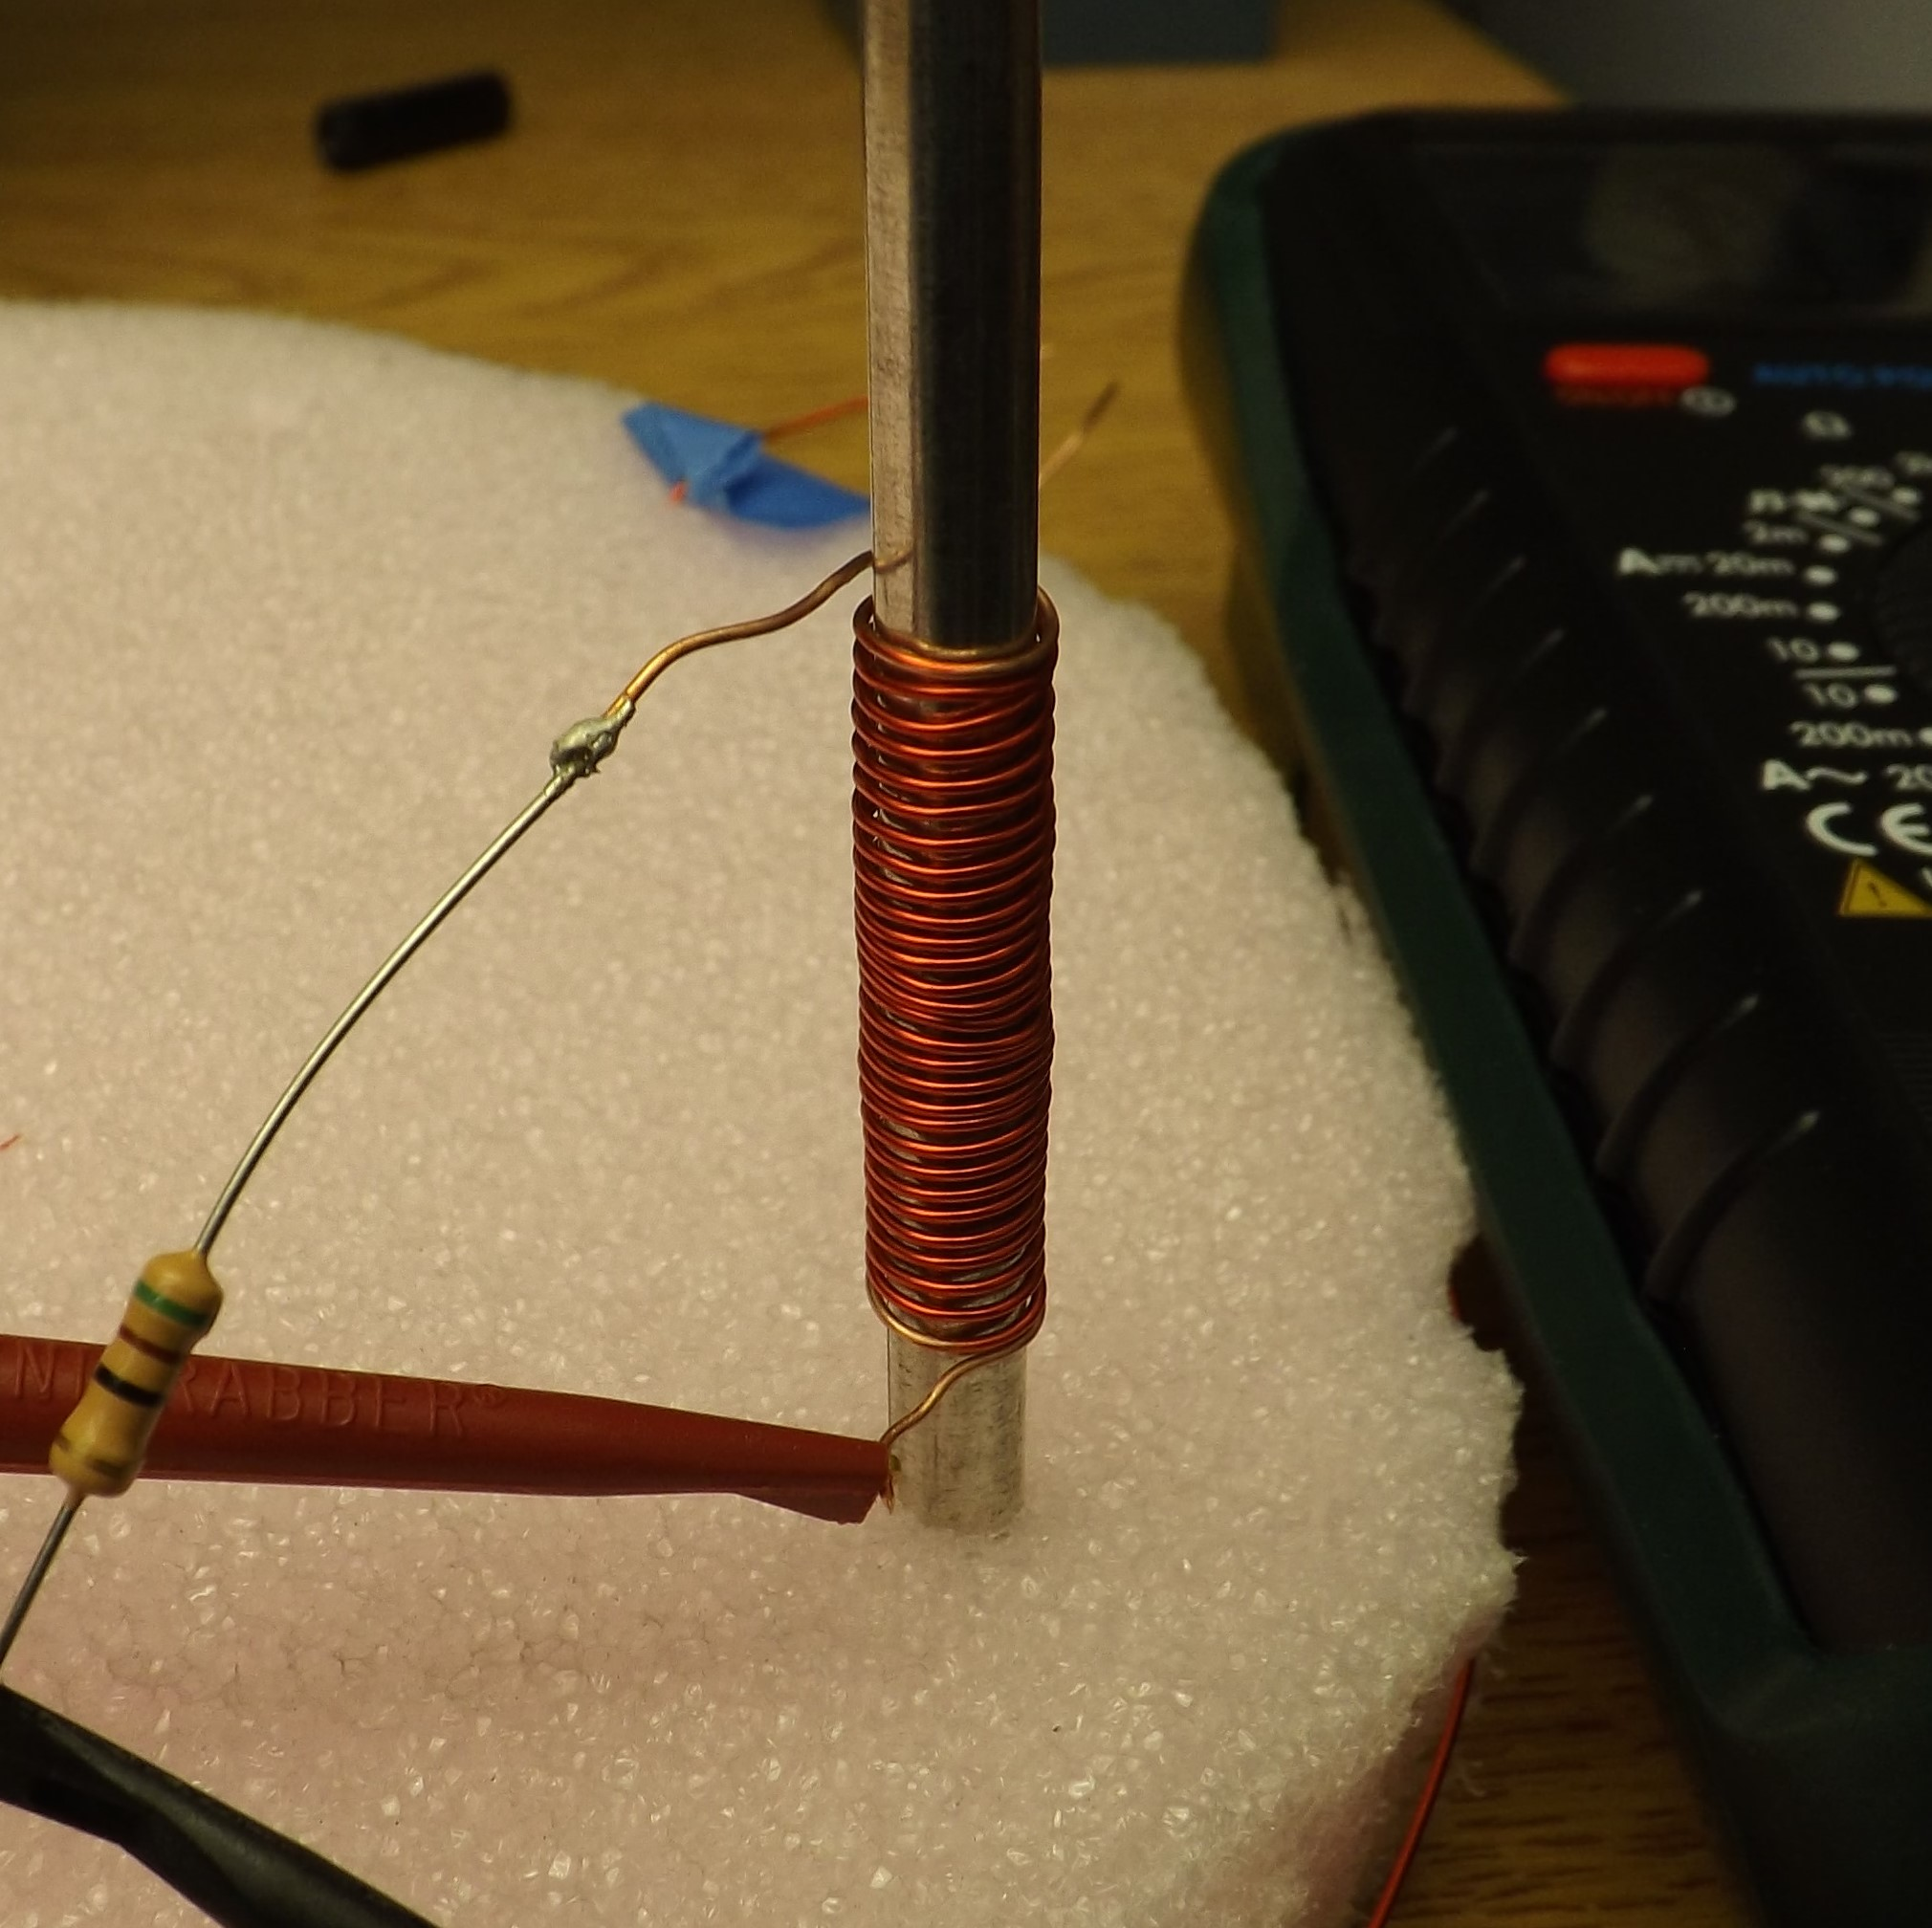
\includegraphics[width=\linewidth]{Inductor-Close-Up.jpg}
    \caption{30-Turn Copper Inductor}
    \label{fig:Inductor}
\end{figure}
\begin{figure}
    \centering
    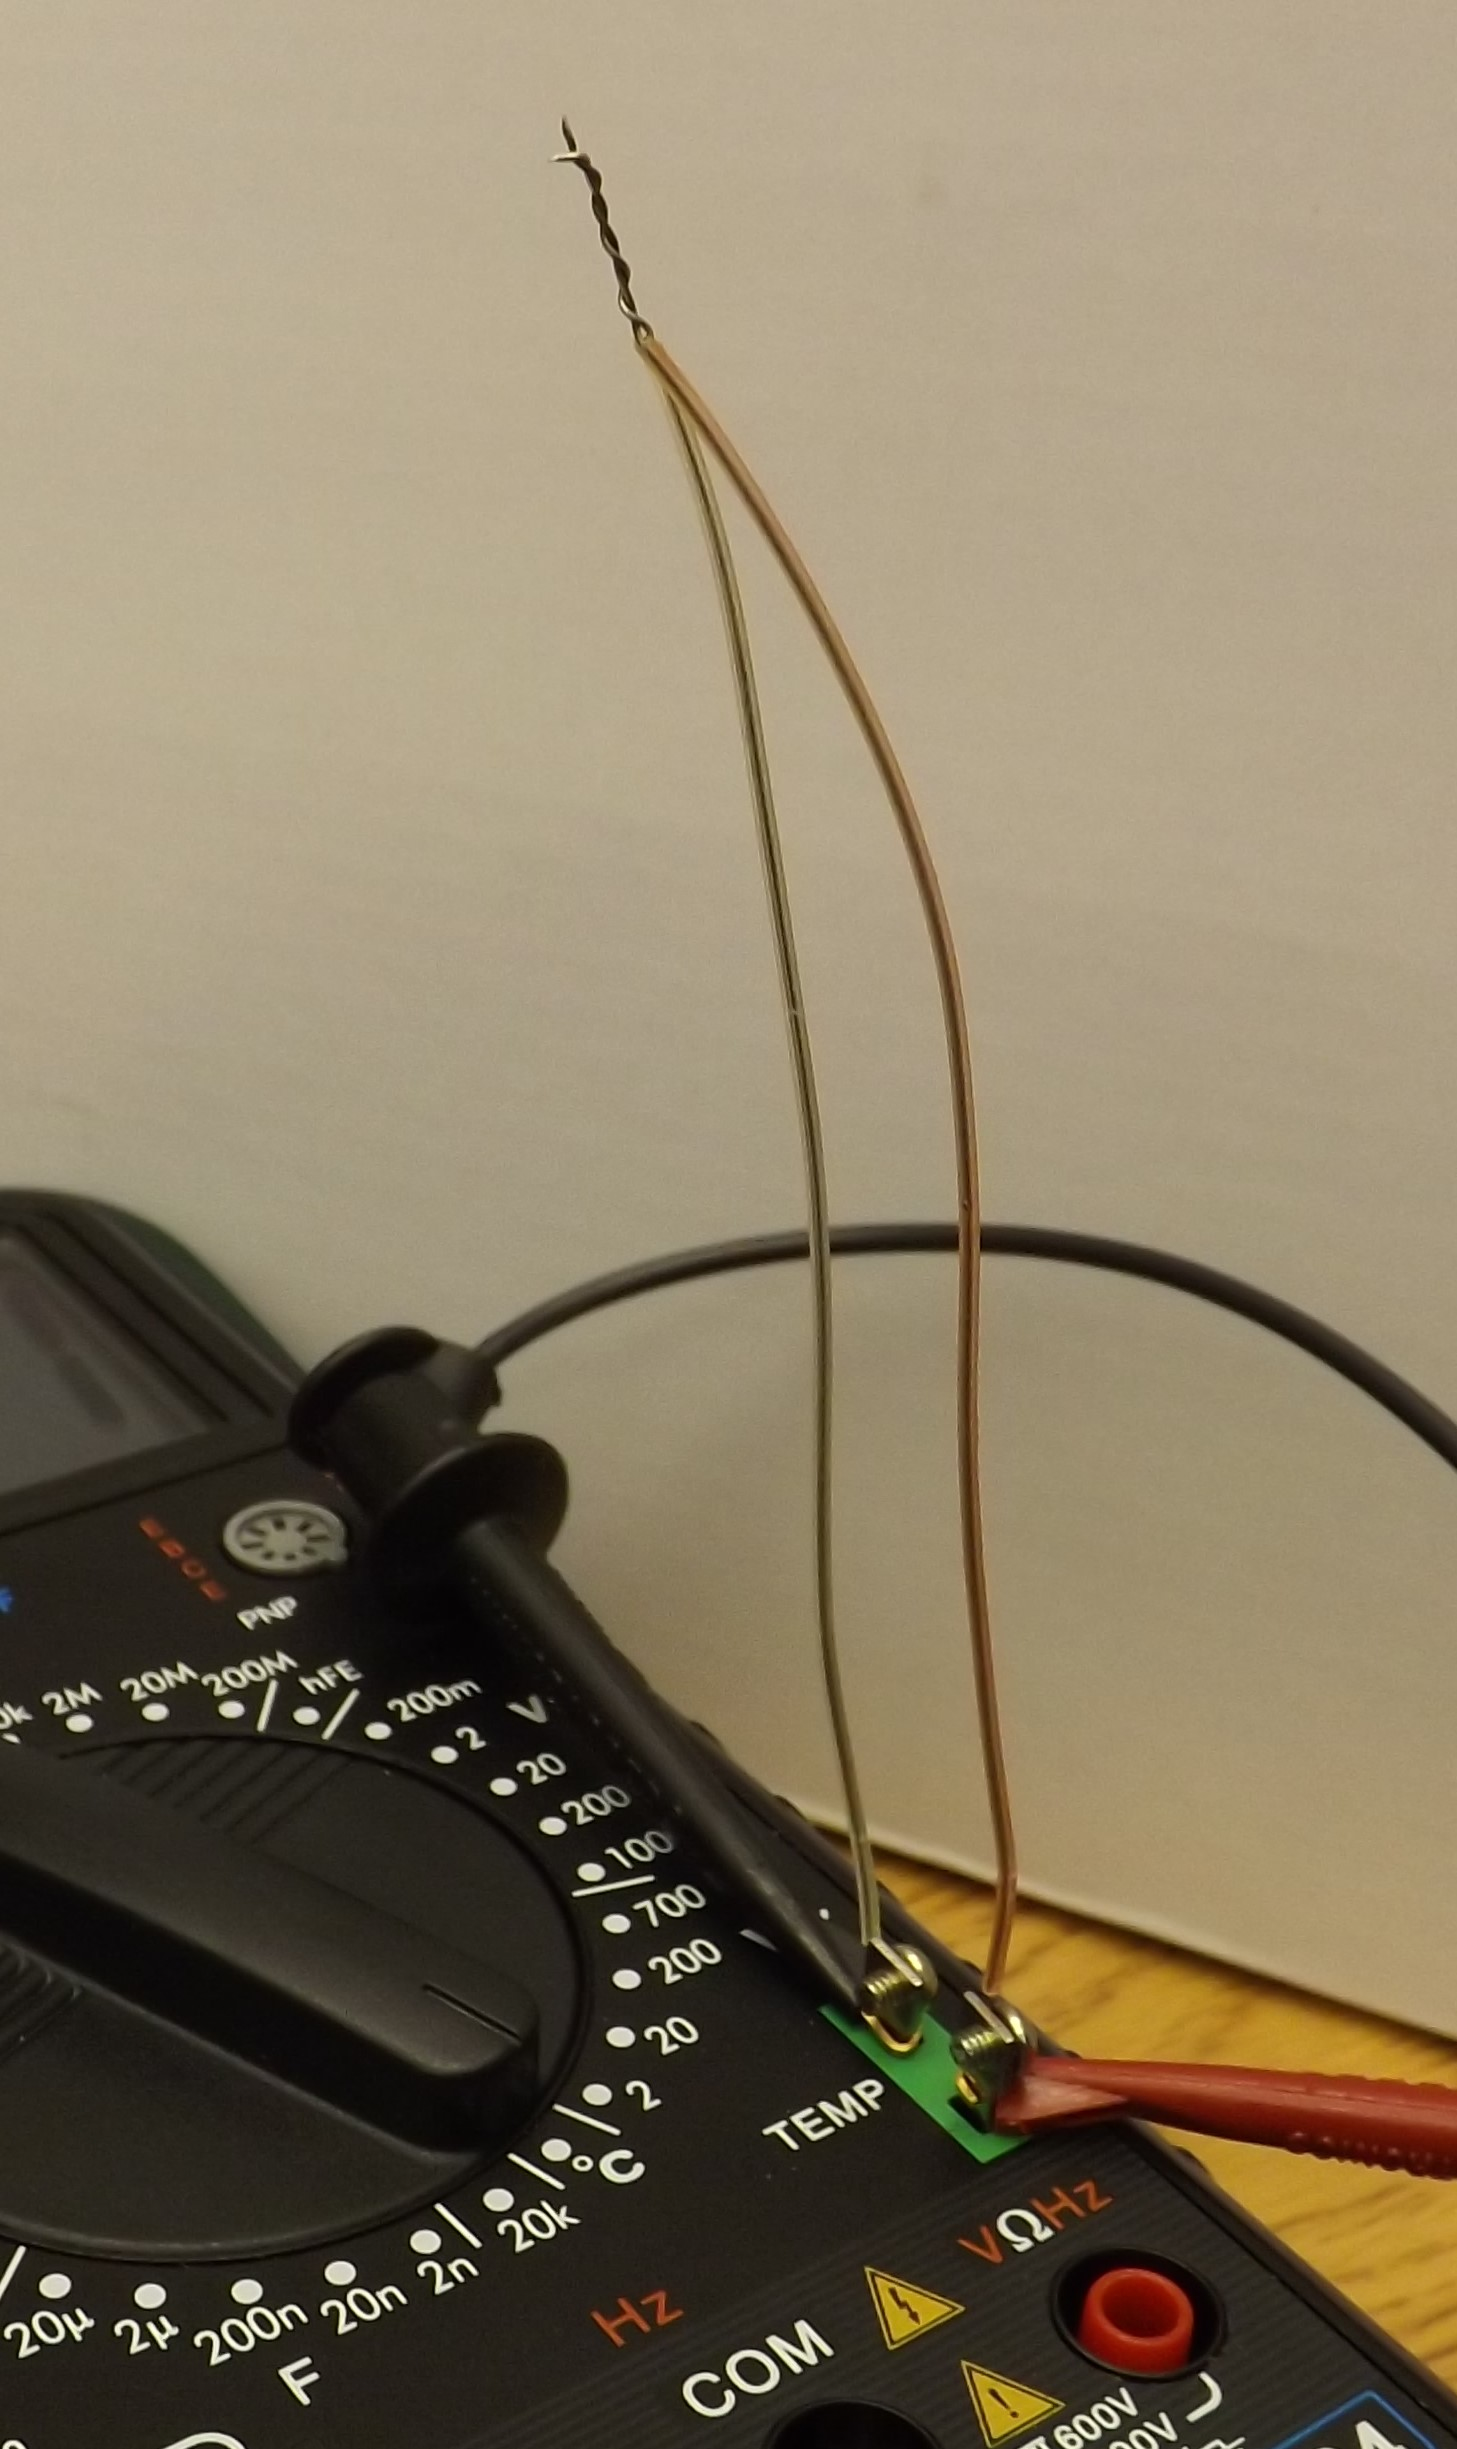
\includegraphics[width=.5\linewidth]{Thermocouple.jpg}
    \caption{Type-K Thermocouple}
    \label{fig:Thermocouple}
\end{figure}
\begin{figure}
    \centering
    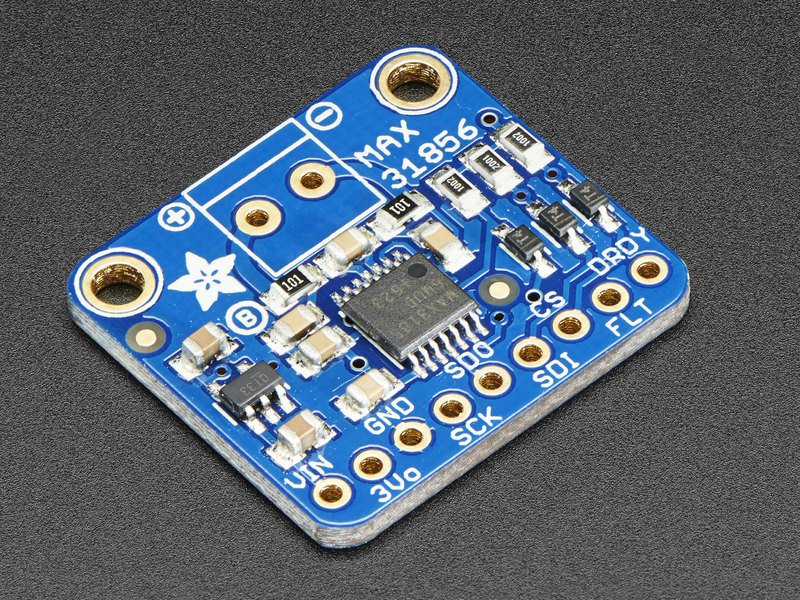
\includegraphics[width=0.75\linewidth]{MAX31856.jpg}
    \caption{MAX31856 Breakout Board}
    \label{fig:MAX31856}
\end{figure}
\begin{figure}
    \centering
    \includegraphics[width=\linewidth]{DPO3034.jpg}
    \caption{Tektronix DPO 3034}
    \label{fig:DPO3034}
\end{figure}
\begin{figure}
    \centering
    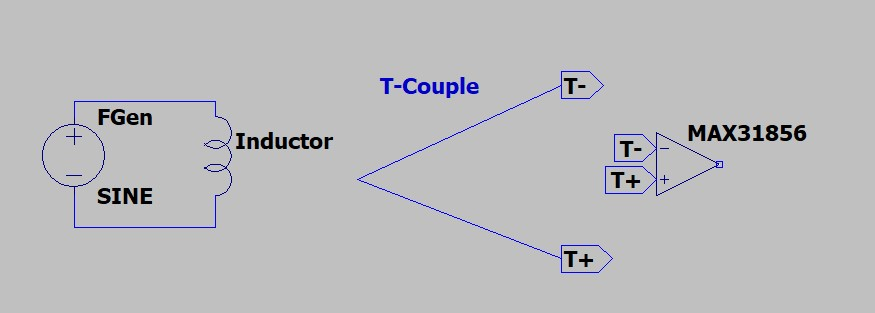
\includegraphics[width=\linewidth]{Block-Diagram.jpg}
    \caption{Experiment Setup Block Diagram}
    \label{fig:Block}
\end{figure}

Using the function generator, we performed a frequency sweep from 10Hz to 70 MHz at 10$V_{pp}$ to see which frequencies were the most apparent on the output. From the sweep, the thermocouple showed the most response at 47Mhz \cref{fig:47mhz,fig:InductorThermocouple,fig:Osci47,fig:Osci47-2}. As is shown in the figures, the thermocouple is showing a 47MHz at 202$mV_{pp}$ signal without being directly connected to the function generator. However, this signal did not translate to a change in the temperature output of the MAX31856. Instead of showing the temperature corresponding to the induced $V_{pp}$ signal as was expected, the thermocouple continued to operate normally, registering real temperate changes that were performed.

\begin{figure}
    \centering
    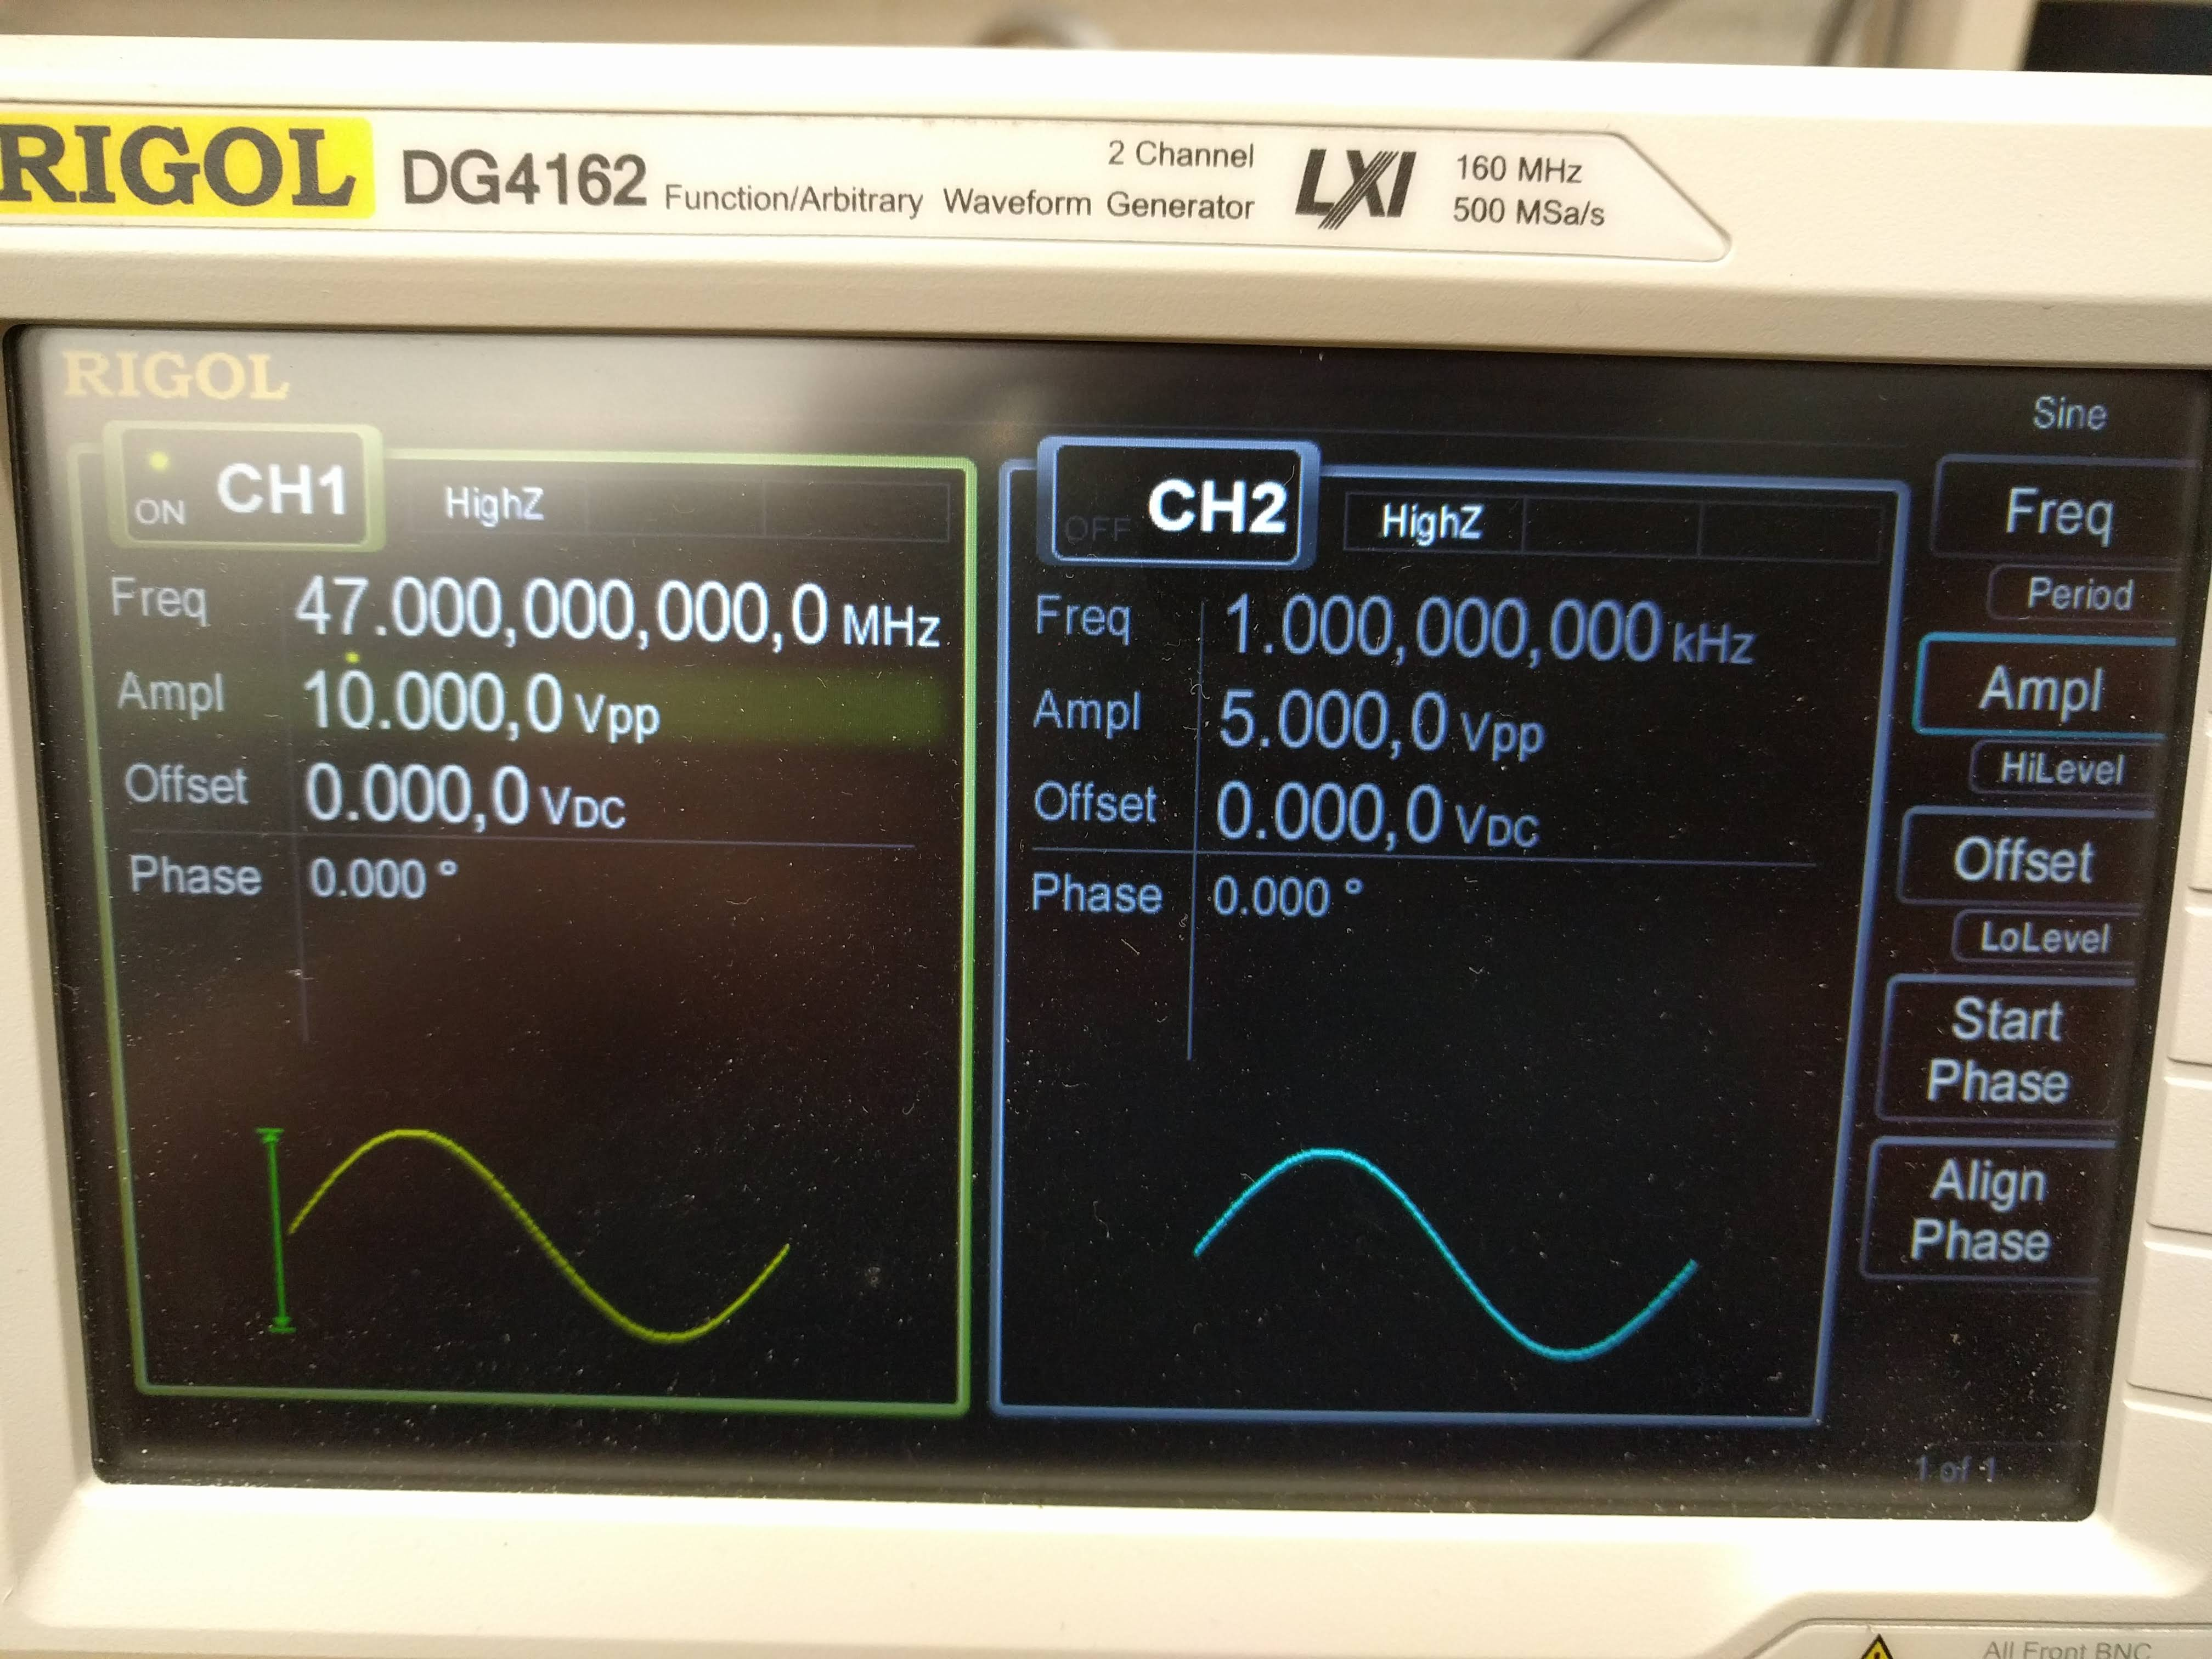
\includegraphics[width=\linewidth]{pictures/47Mhz.jpg}
    \caption{Function Generator Operating at 47MHz}
    \label{fig:47mhz}
\end{figure}
\begin{figure}
    \centering
    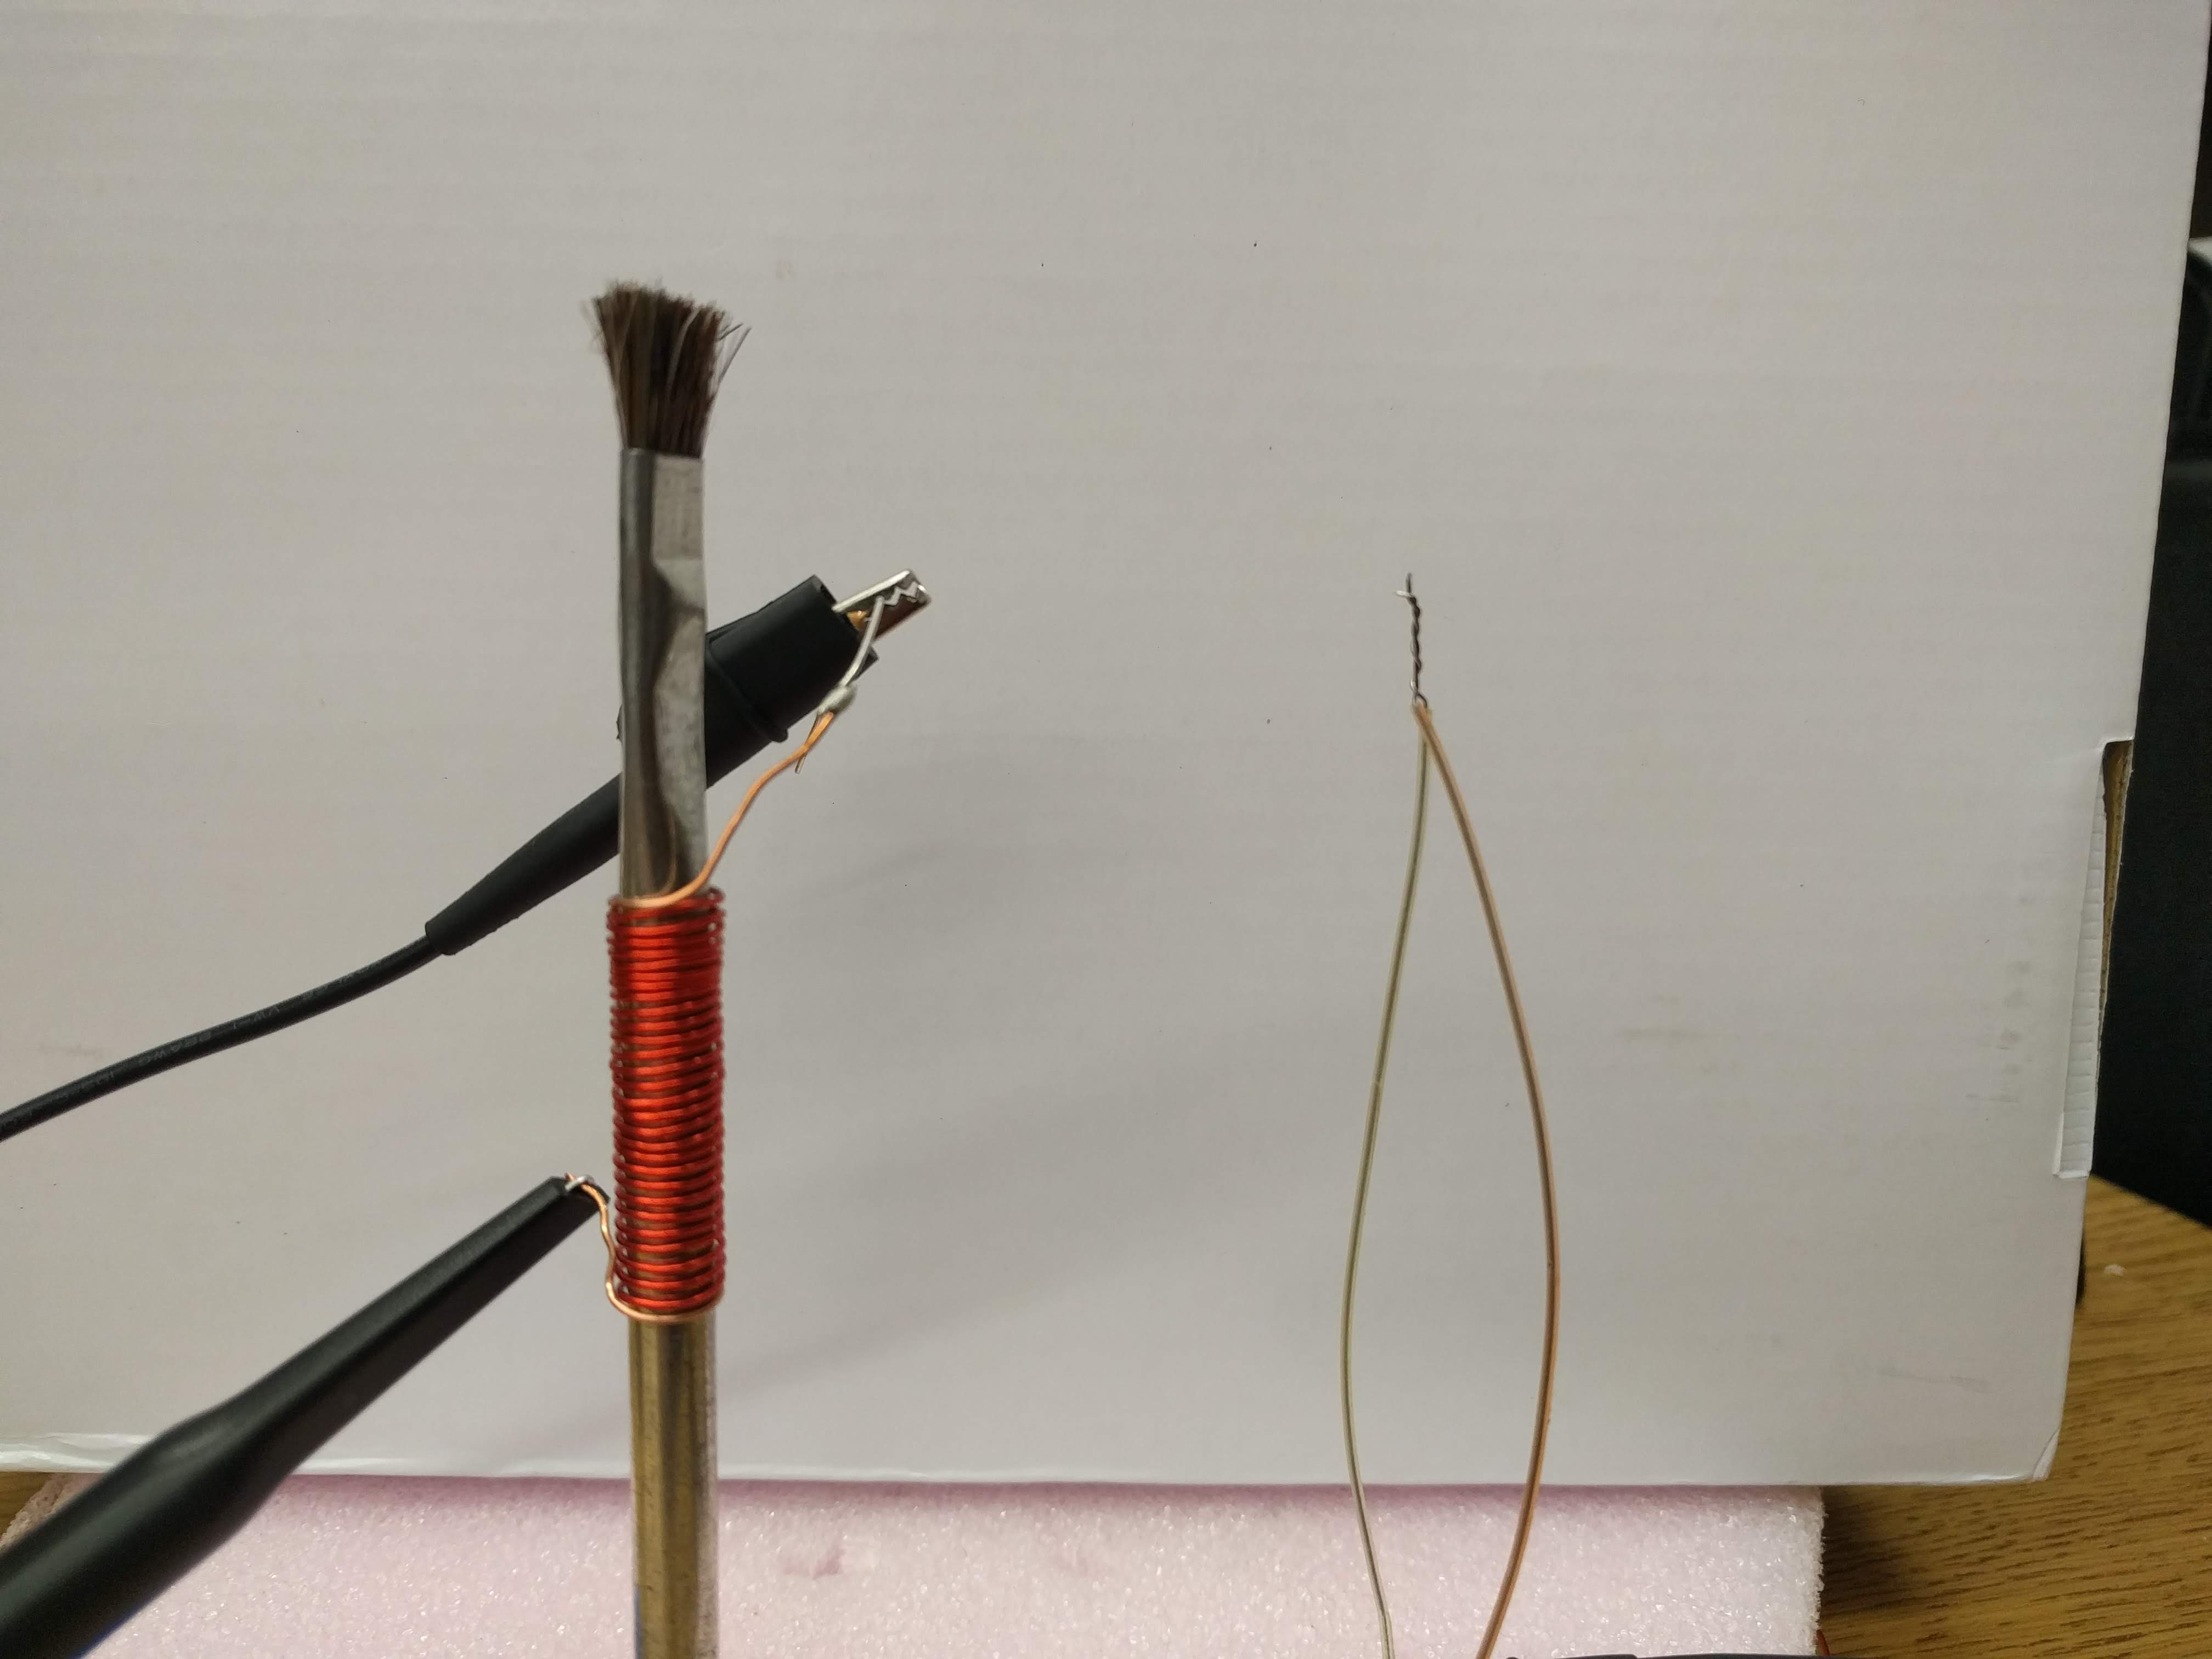
\includegraphics[width=\linewidth]{pictures/Inductor+TCouple.jpg}
    \caption{Inductor and Thermocouple During the Experiment}
    \label{fig:InductorThermocouple}
\end{figure}
\begin{figure}
    \centering
    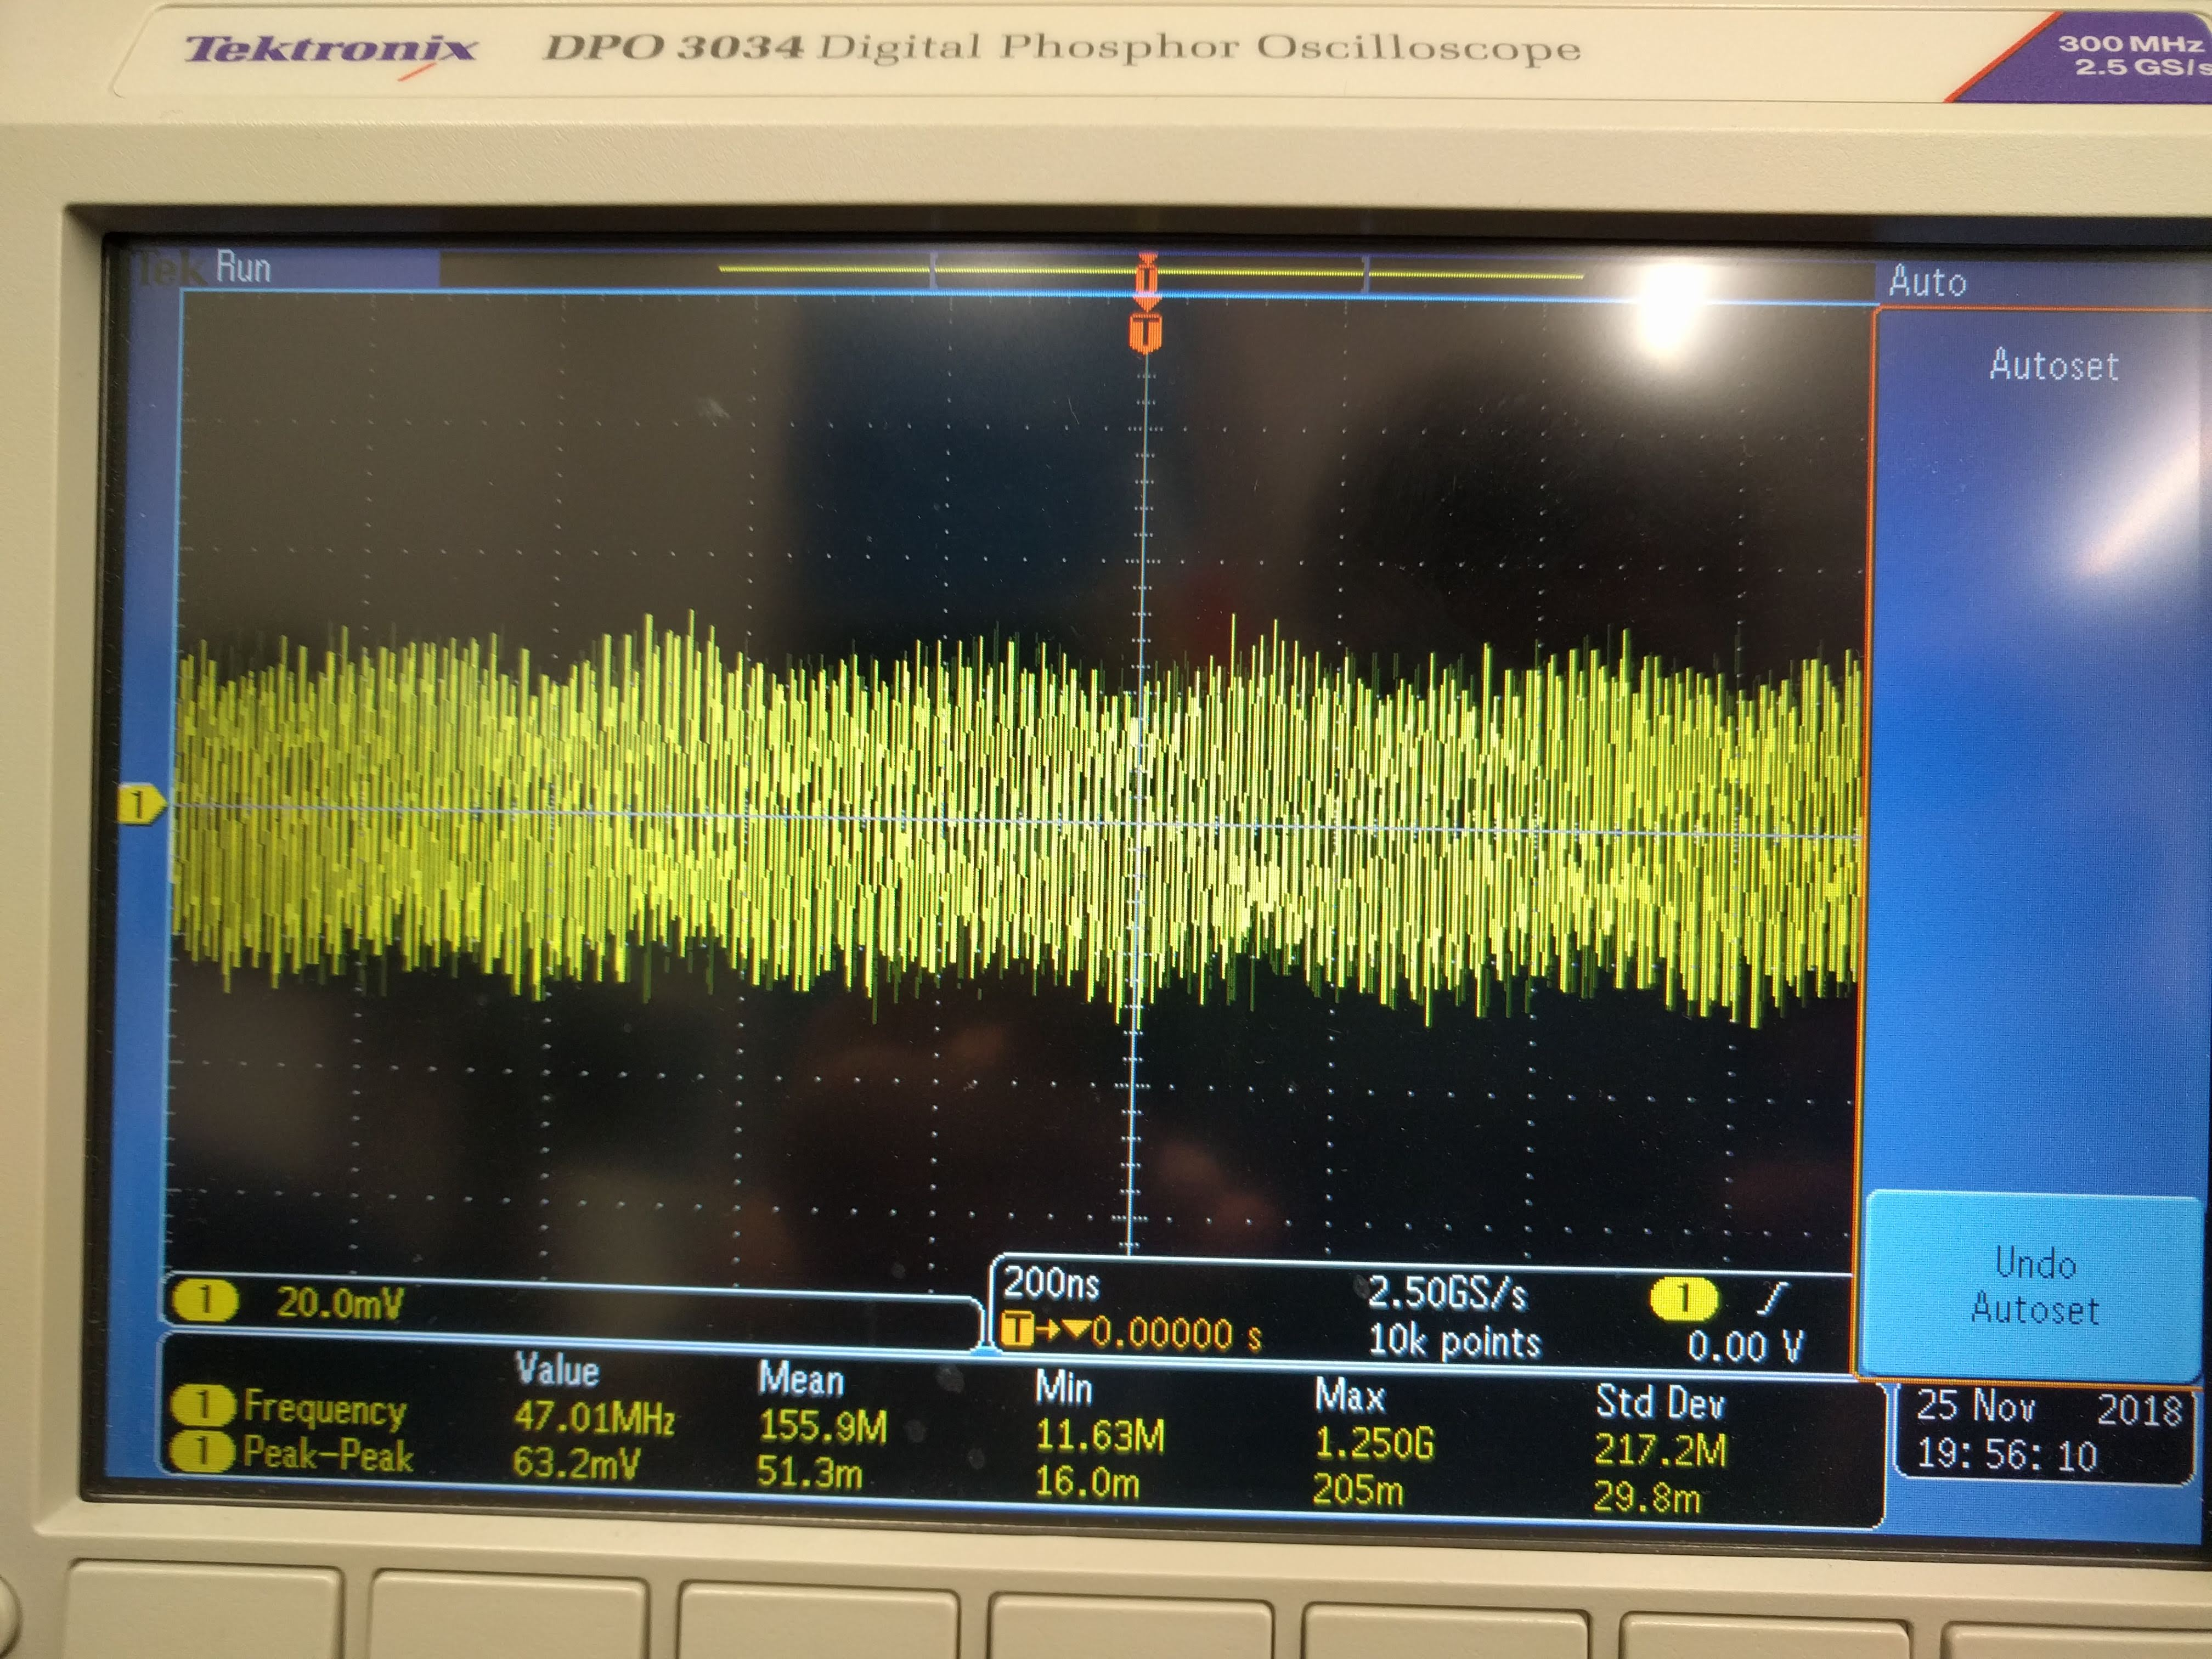
\includegraphics[width=\linewidth]{pictures/Osci-47.jpg}
    \caption{Oscilliscope Showing Induced Waveform}
    \label{fig:Osci47}
\end{figure}
\begin{figure}
    \centering
    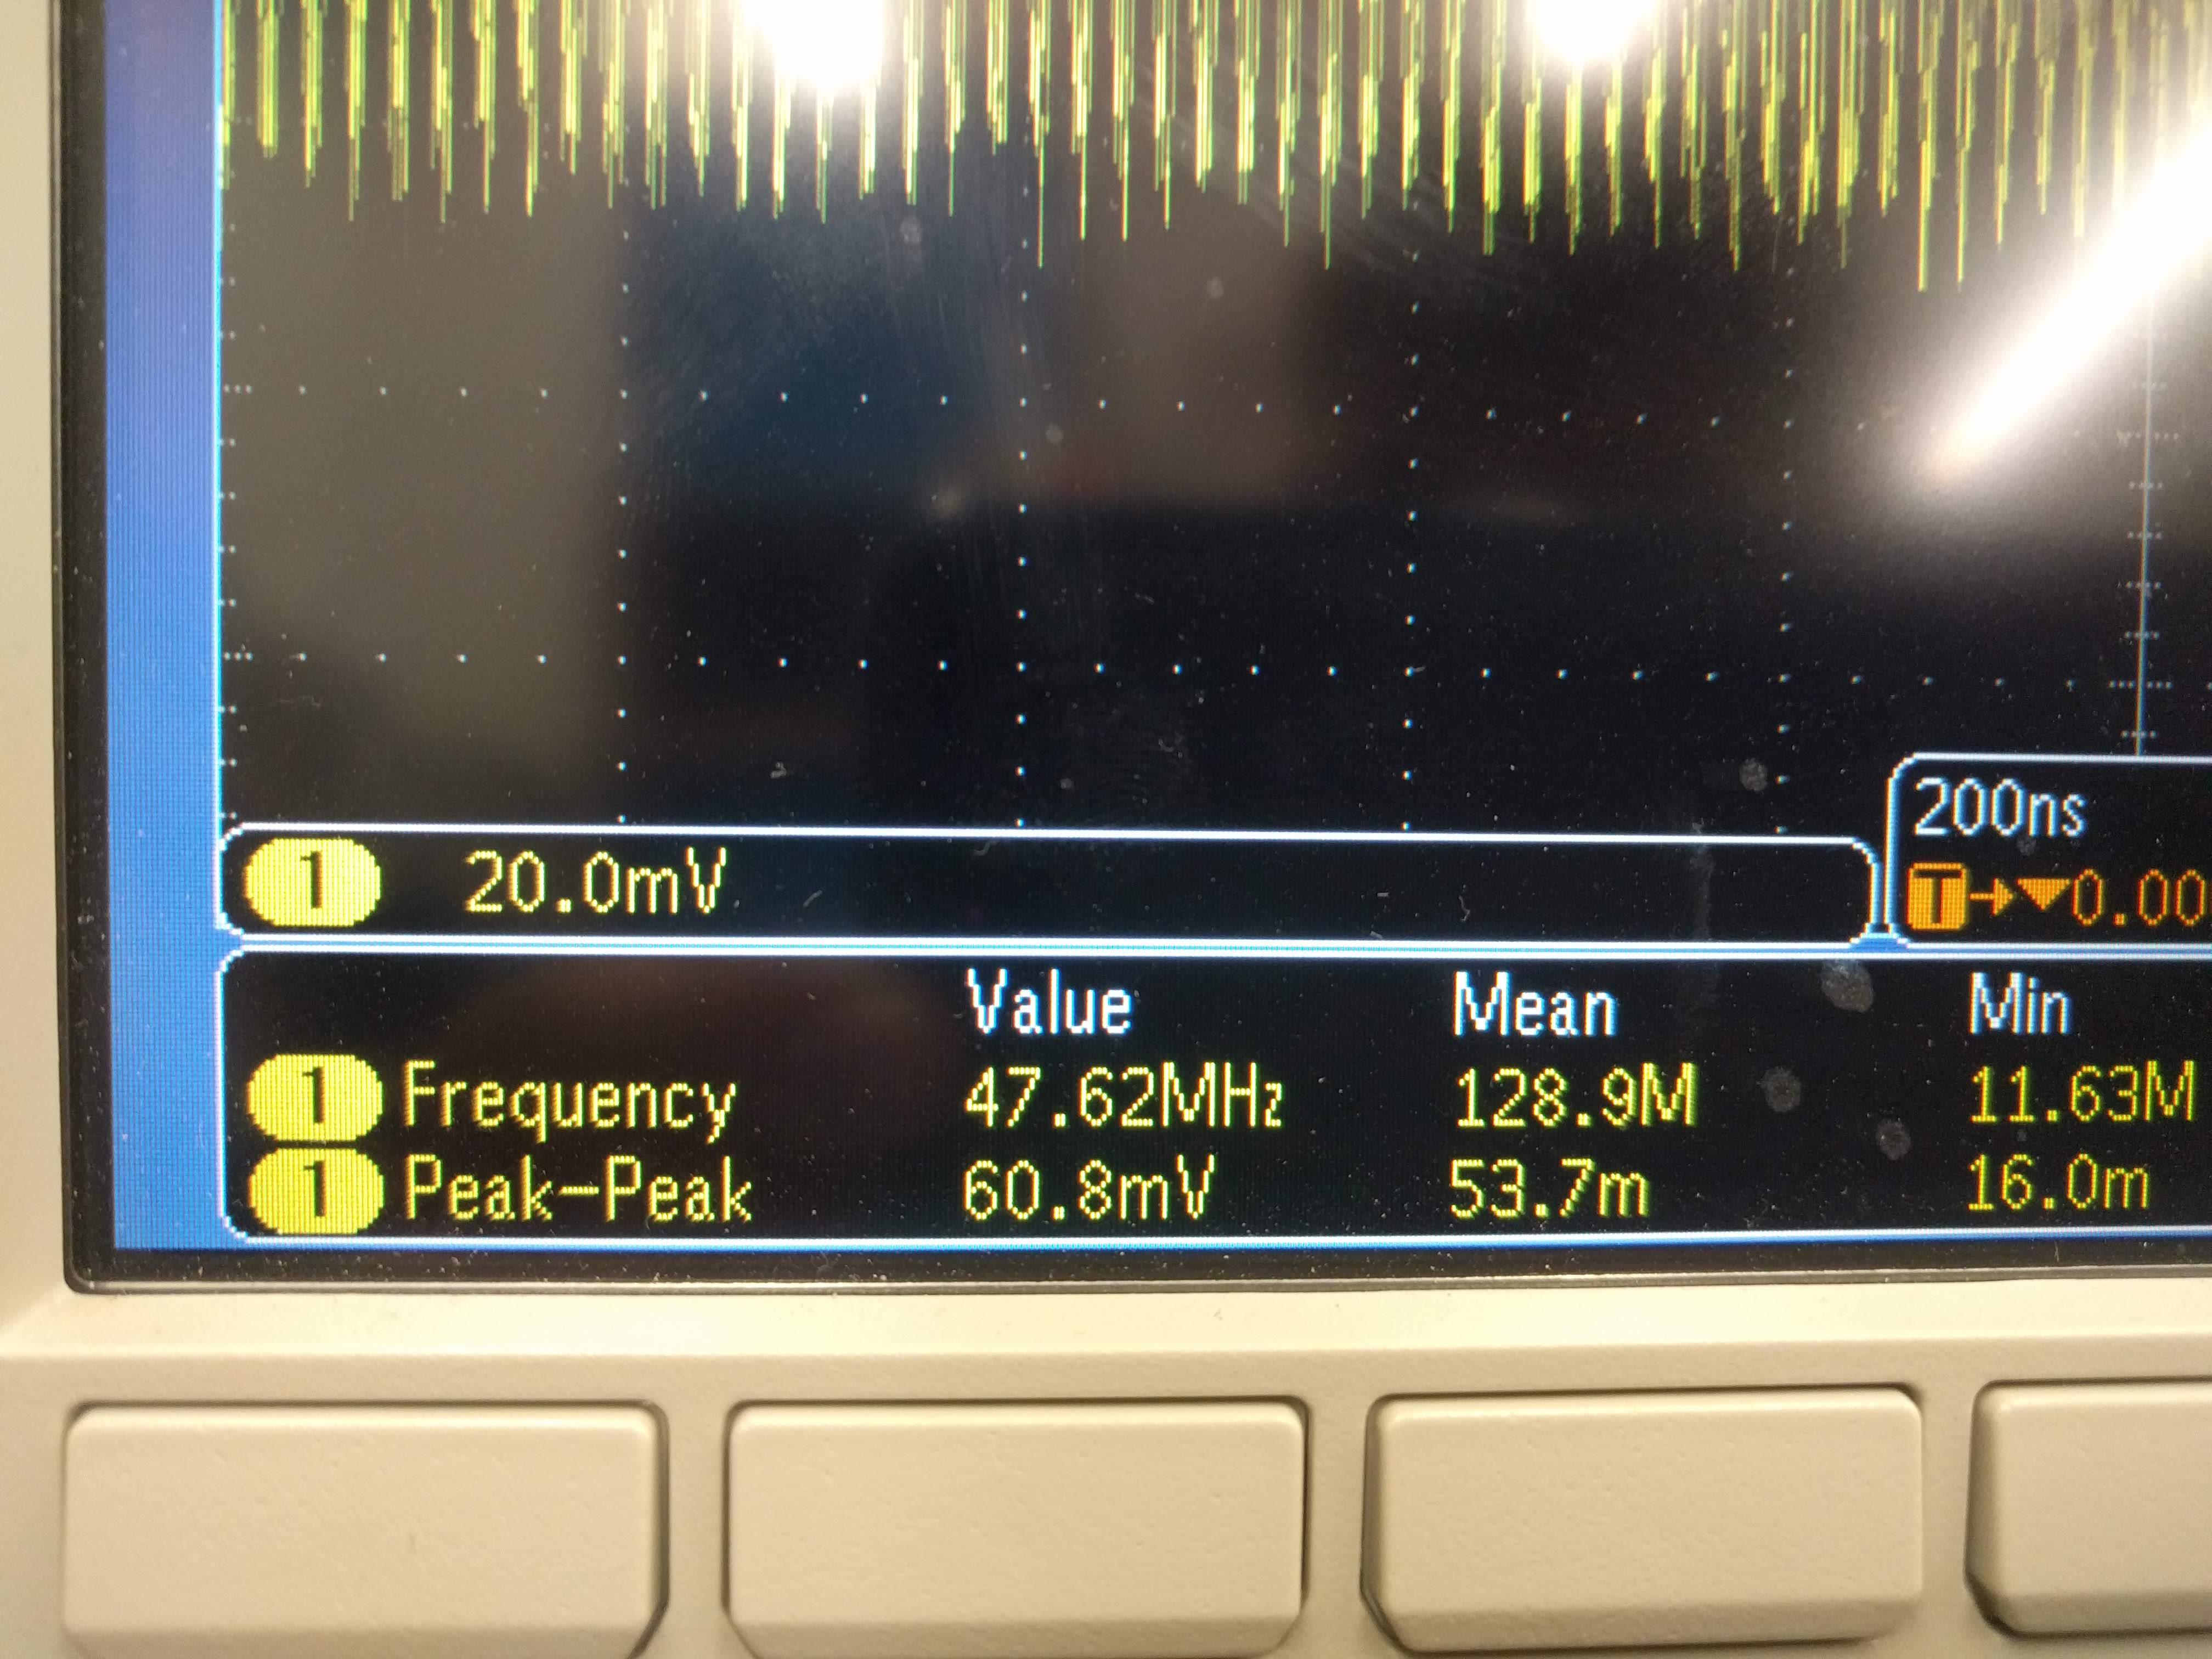
\includegraphics[width=\linewidth]{pictures/Osci-47-2.jpg}
    \caption{47MHz Waveform on Thermocouple}
    \label{fig:Osci47-2}
\end{figure}

The next experiment done was observing the effects of multiple emitters operating at differing frequencies on the thermocouple output. Here, we simply added another inductor connected to the second output of the function generator. We kept the first emitter constant at 47 MHz while stepping the second from 42-52Mhz in increments of 1Mhz. The results were that the induced signal on the thermocouple was the constructive/destructive interference between the two input signals. An example is shown in \cref{fig:fgencombo,fig:InductorThermocoupleCombo,fig:OsciHarmonic}. Once again, the induced signal did not translate to real temperature output interference. Instead, the thermocouple continued to operate normally. 

\begin{figure}
    \centering
    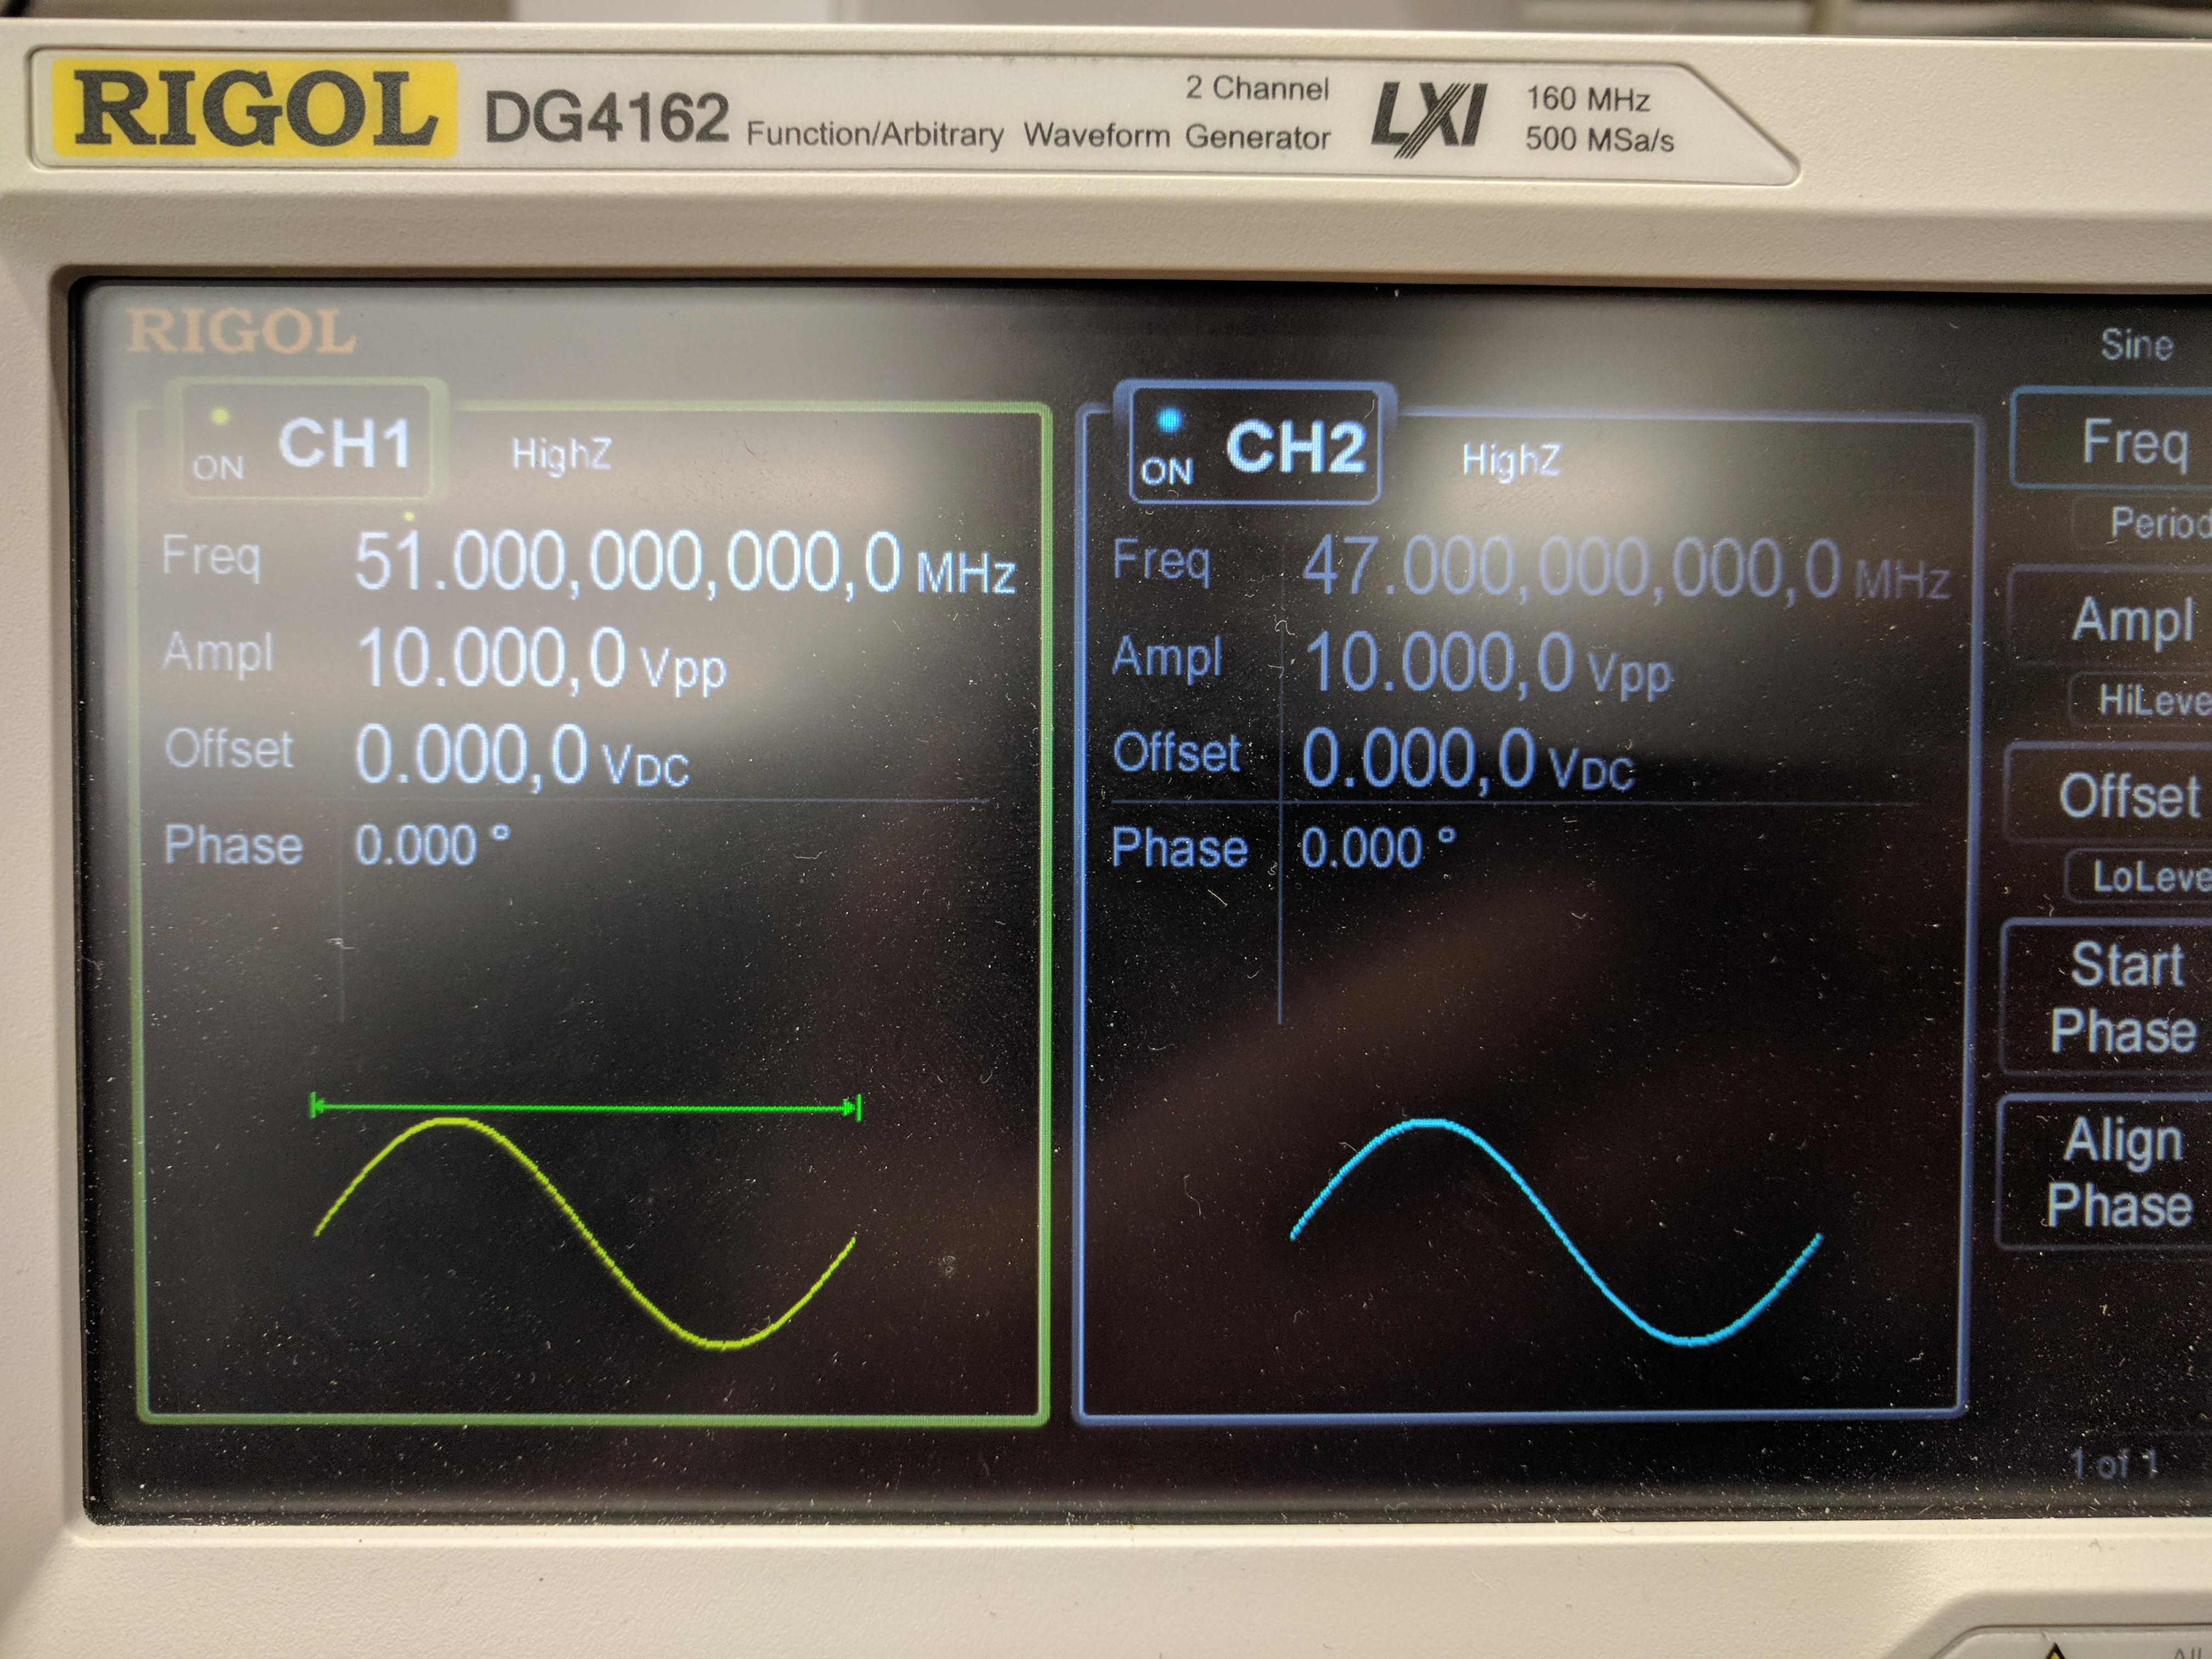
\includegraphics[width=\linewidth]{pictures/FGen-Combo.jpg}
    \caption{Function Generator Operating at Two Frequencies}
    \label{fig:fgencombo}
\end{figure}
\begin{figure}
    \centering
    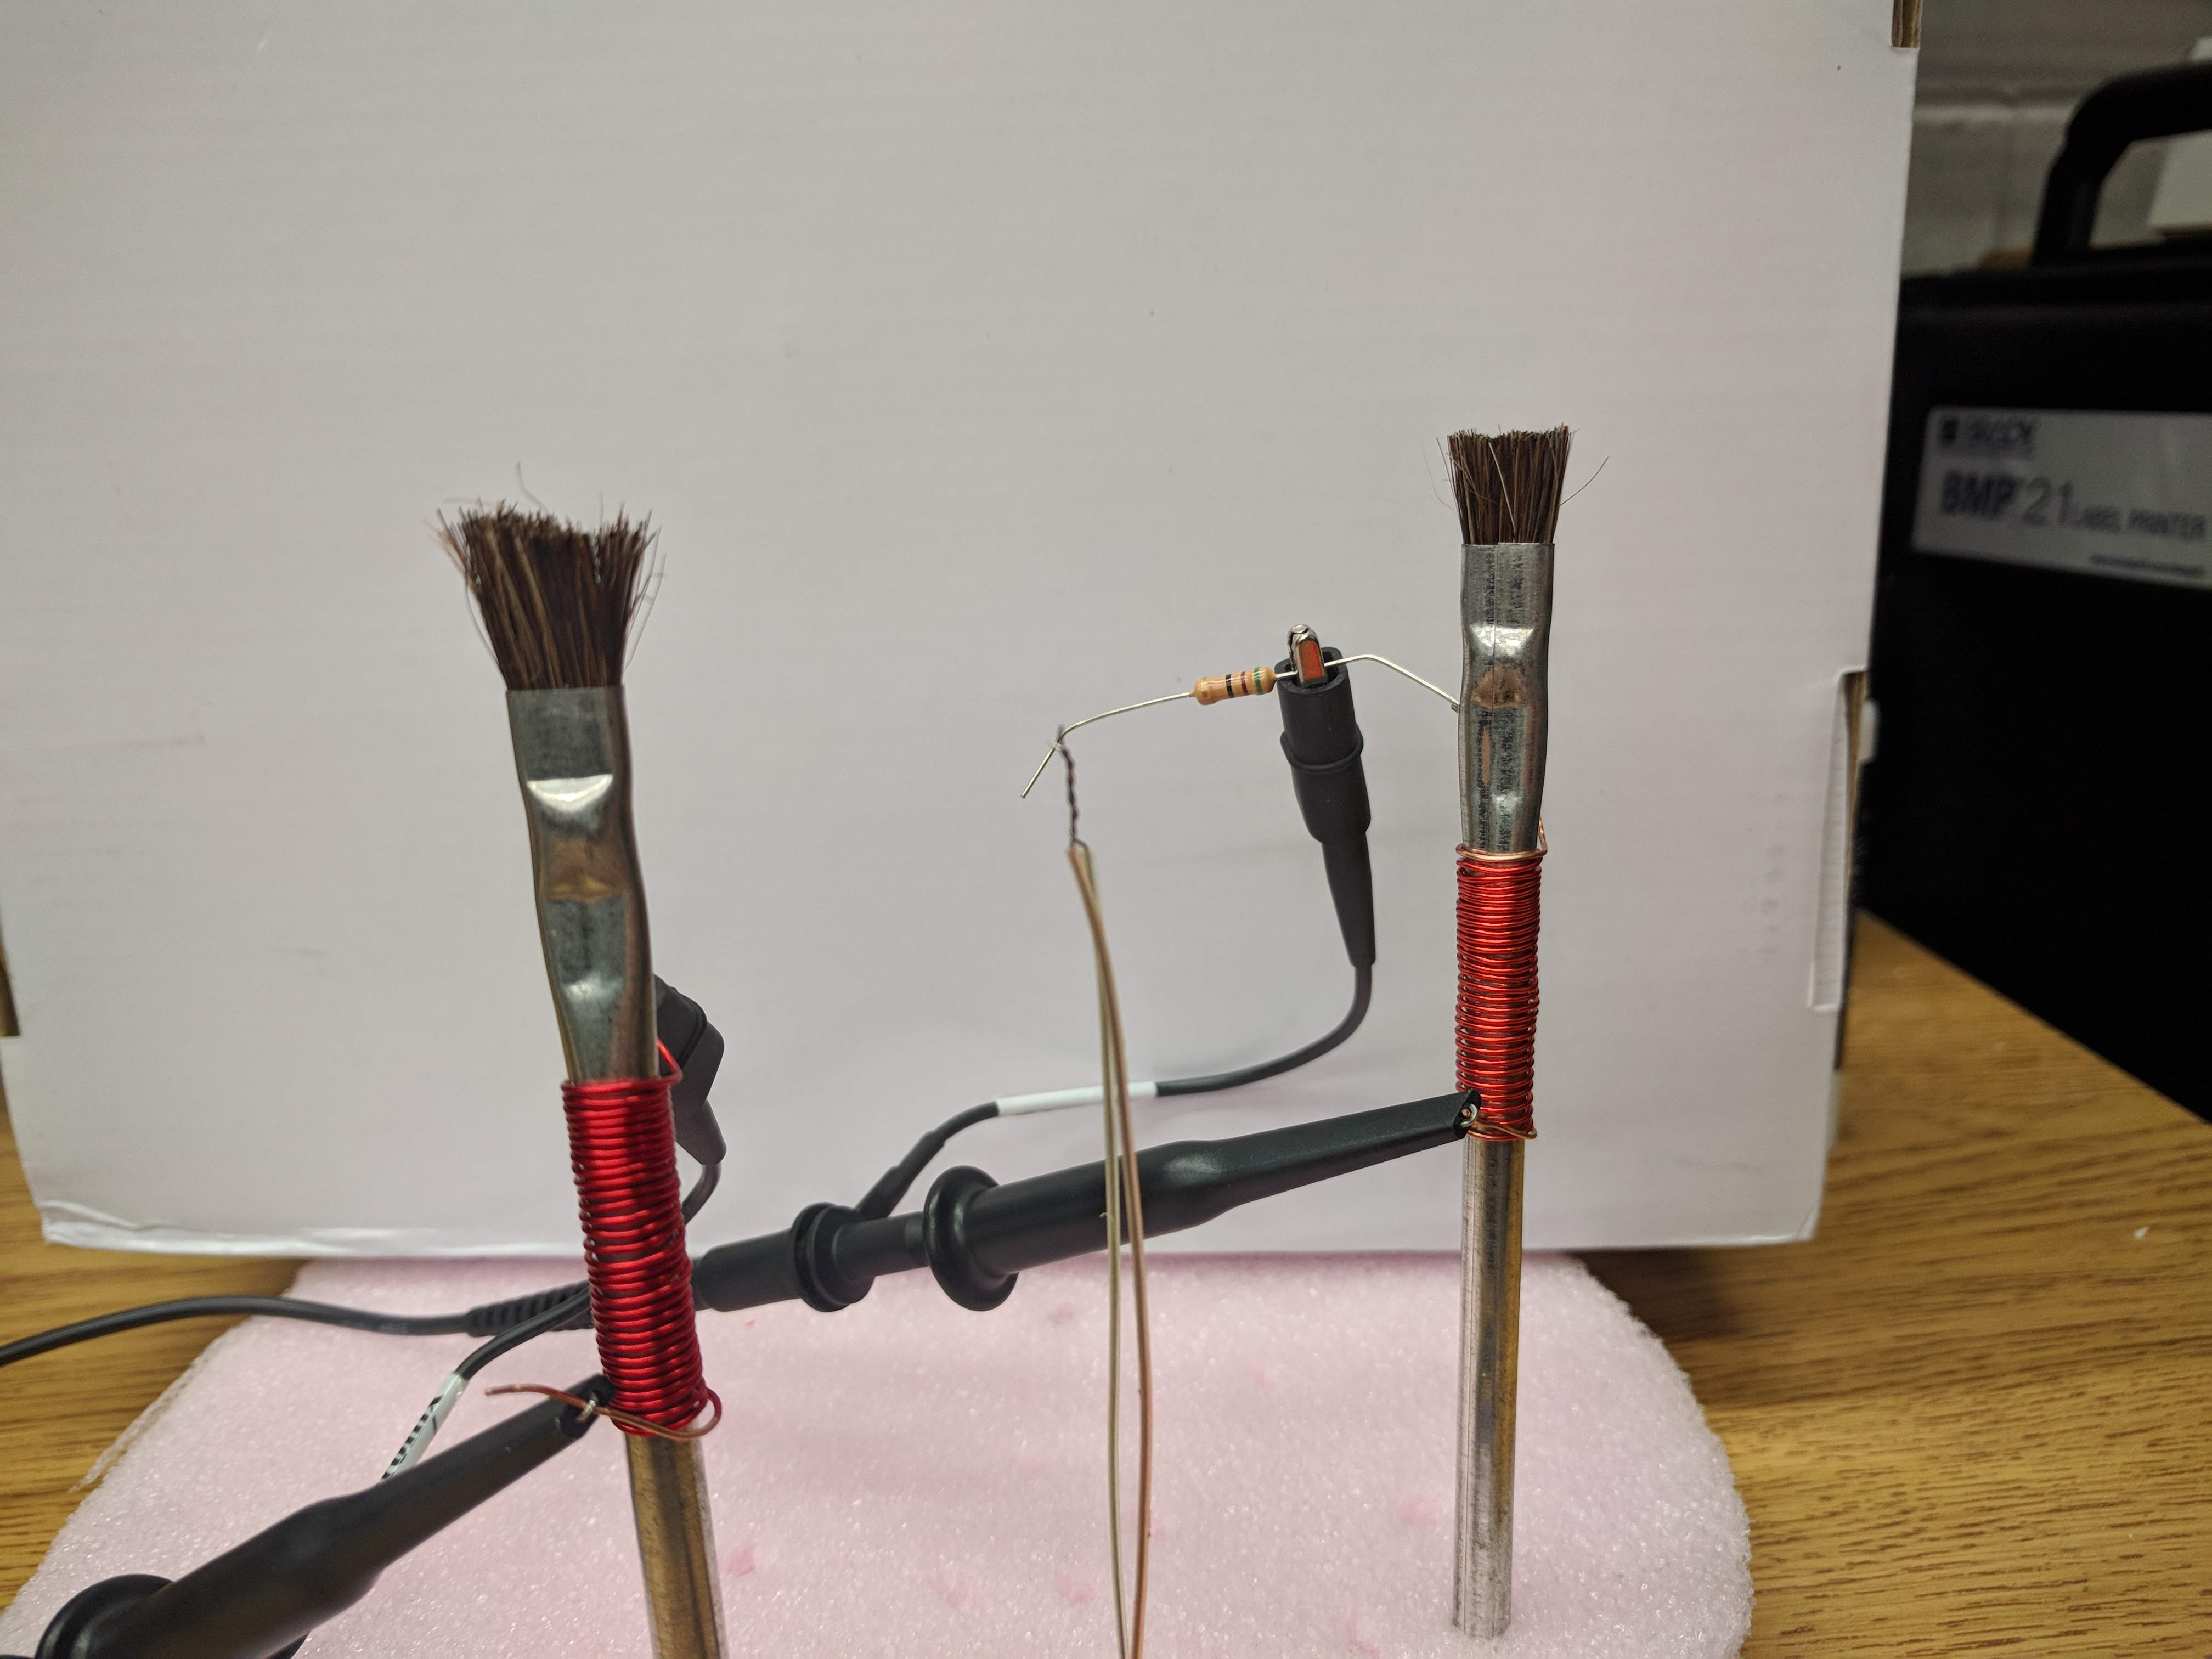
\includegraphics[width=\linewidth]{pictures/Tcouple-Combo.jpg}
    \caption{Inductor and Thermocouples During the Experiment}
    \label{fig:InductorThermocoupleCombo}
\end{figure}
\begin{figure}
    \centering
    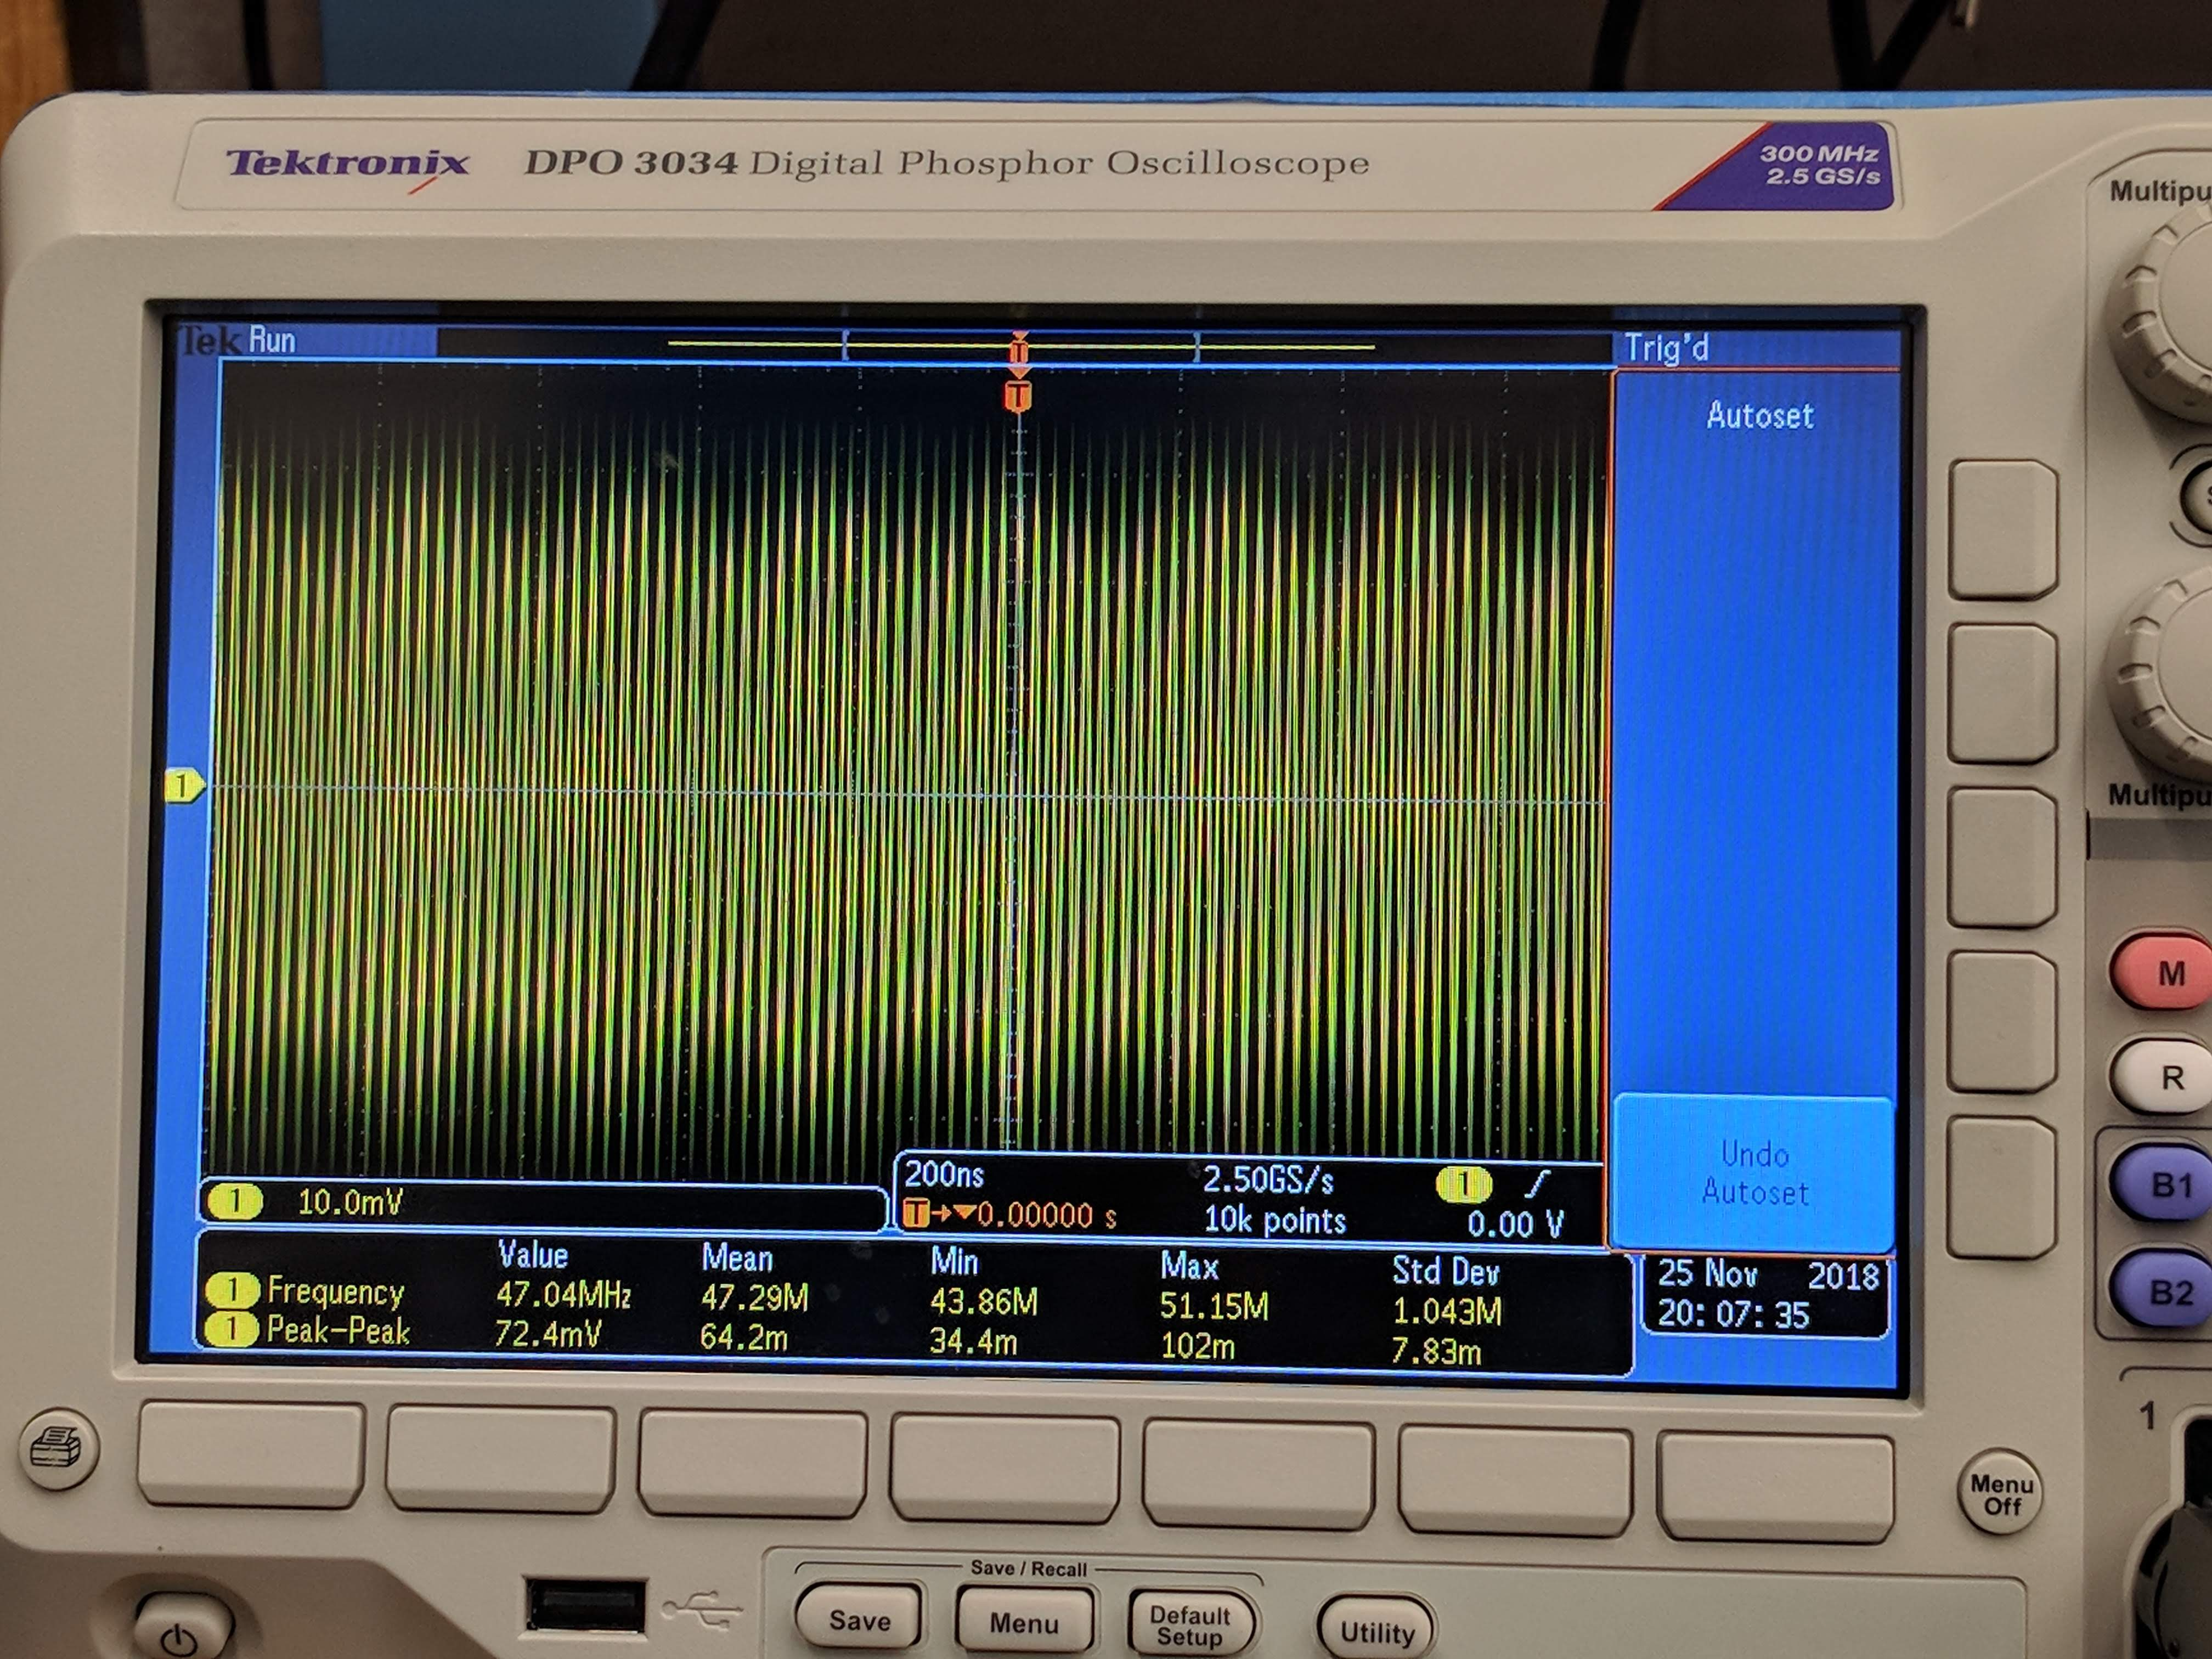
\includegraphics[width=\linewidth]{pictures/Harmonic.jpg}
    \caption{Oscilloscope Showing 47Mhz Harmonic as a Result of Multiple Inductors}
    \label{fig:OsciHarmonic}
\end{figure}

\subsection{What went wrong}\label{wwdw}
From the experiments we were able to learn two things: inducing an \ac{ac} signal on a thermocouple using \ac{emi} is simple at the right frequencies, and that induced signal was not enough to translate to temperature interference. 
On its own, an \ac{ac} signal would not be enough to change the output temperature. This is because the mean value of any sine wave is zero. So, no change in what the MAX31856 was measuring would be seen without some \ac{dc} offset being produced. However, the induced signals from the experiments never had a \ac{dc} offset, thus explaining the lack of interference. 

Another aspect of creating a \ac{dc} offset is that all wires (including the thermocouple itself) have an intrinsic capacitive component. This can result in a rectifier that can convert the induced \ac{ac} signal to a constant \ac{dc} value. In the case of the MAX31856, three additional capacitors are added to the circuit which are meant to reduce noise across the thermocouple wires. A SPICE model derived from the MAX31856 datasheet is shown in \cref{fig:SPICE}. The 0.735V on T- is a result of a bias output from the MAX31856, while V1 is a model of the induced signal on the thermocouple. After a transient simulation \cref{fig:SIM}, the amplitude of the induced signal was reduced to ~70 $\mu V_{pp}$ with no \ac{dc} offset, not appropriate for creating a faulty temperature.  

\begin{figure}
    \centering
    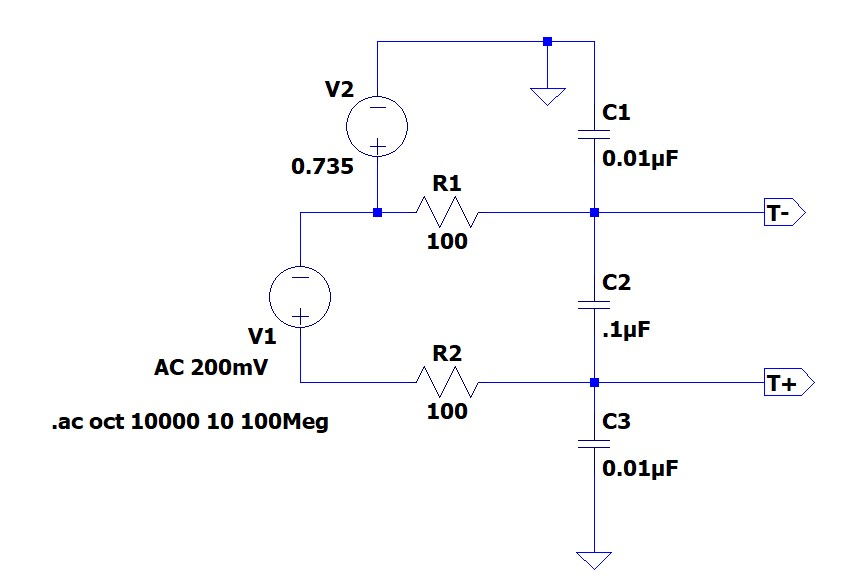
\includegraphics[width=\linewidth]{pictures/SPICE.jpg}
    \caption{SPICE Model of the MAX31856 Interface}
    \label{fig:SPICE}
\end{figure}
\begin{figure}
    \centering
    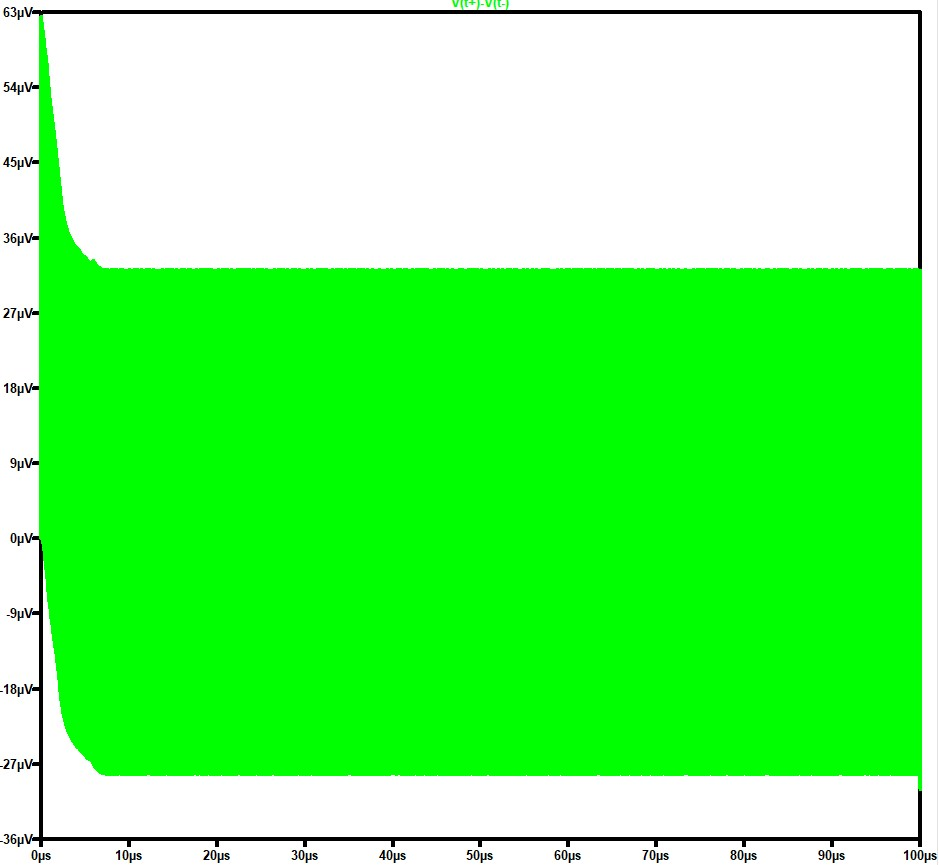
\includegraphics[width=\linewidth]{pictures/Time-Plot.jpg}
    \caption{Transient Simulation of the MAX31856 Interface}
    \label{fig:SIM}
\end{figure}

The simulated frequency response graph \cref{fig:BODE} supplies more evidence that our methods were not appropriate for creating a temperature output change. As the frequency of the induced signal increases, the response of the circuit becomes exponentially smaller. At the frequency where our experiments were operating (47MHz) the response of the MAX31856 input circuit is ~-90dB. This negative response makes creating any \ac{dc} component in the final signal very difficult.
A final mistake in our approach was the assumption that interference targeted at the thermocouple would be enough to cause output interference. There are multiple attack points just within the simple thermocouple experiments that could have been exploited. First, the MAX31856 is an IC device that has its own sensors (i.e. cold junction temperature sensor) that can be interfered with. In addition, attacks on the SPI controller as well as the microcontroller inside of device could have been explored.

\begin{figure}
    \centering
    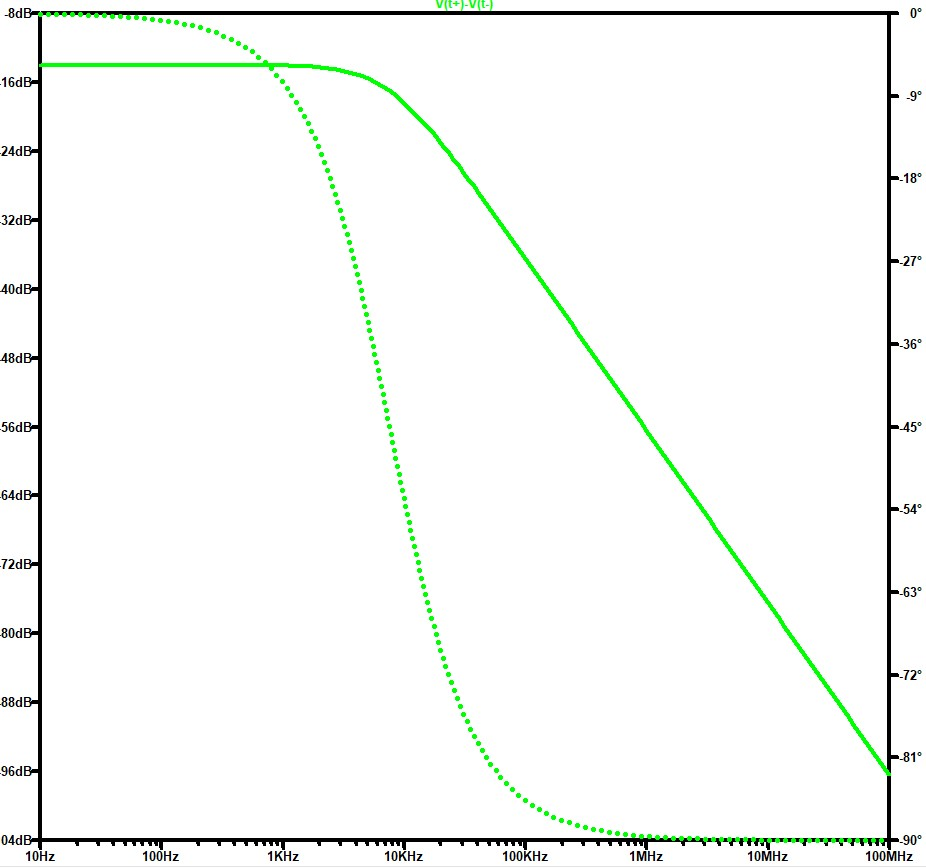
\includegraphics[width=\linewidth]{pictures/Bode.jpg}
    \caption{Bode Plot of MAX31856 Interface}
    \label{fig:BODE}
\end{figure}

\section{Software Implementation}\label{swi}
\subsection{Model Creation}\label{model-creation}
Both the simulation as well as the controller rely on a steady-state model of the thermocouple to produce realistic looking values. To do this, we used our K-Type thermocouple as a sample source for a statistical model. First, we took continuous reading over a half hour where the thermocouple and MAX31856 were at room temperature. Using Mathematica, we fit a distribution to the samples and created the inverse \ac{cdf} \cref{inverse-cdf-tcouple}. Through the inverse \ac{cdf} sampling method, we could then use the resulting function as the source for our simulation. 

\begin{equation}\label{inverse-cdf-tcouple}
\begin{split}
t = x - 0.0620762 \log({-1 + 1/y}),
\end{split}
\begin{split}
t \text{- Temperature}\\
x \text{- Mean Temperature}\\
y \text{- Random number (0, 1]}
\end{split}
\end{equation}

\subsection{Controller}
To try to mitigate the effects of induced errors a rolling average was implemented in \cref{thermocouple-controller}. In addition, an upper bound and lower bound for the allowable values of the thermocouple were implemented; if the value read from the thermocouple is outside of this range, the model discussed in \cref{model-creation} is used to calculate an approximate valid value to be stored in the list of values used to calculate the rolling average.

\subsection{Simulation}
To effectively simulate the hardware that was tested several things were needed. Firstly the simulator needed to emulate the functionality of the MAX32 thermocouple that was interfaced with by the arduino. Secondly, the simulator needed the ability to read a series of temperature values from an input file and correctly pass those along to the controller. Following proper implementation of this, functionality was added to include the ability for the simulator to modify the values that were read from the input file to simulate a thermocouple that was being attacked. This was done by forcing the values to either a lower bounded range or an upper bounded range, emulating the extreme voltages that might be induced in the device. This code is available in \cref{thermocouple-simulator}. \Cref{thermocouple-simulator-h} is the header file used to define some of the values used in the simulator.

\section{Discussion}\label{disc}
The controller code can be run on either an Arduino or with the simulator included. This code is shown in \cref{thermocouple-controller}. All of the code written for this design and simulator, as well as a Makefile and README of how to use it can be found on \href{https://github.com/RSAkidinUSA/tc-volt-check}{github}.

\section{Future Work}\label{fut}
Future work would focus primarily on expanding the attack surfaces that were used for interference. As discussed in the previous section, the frequency response of the breakout circuit of the MAX31856 prevented high frequencies from being effective. In addition, alternate parts of the system need to be probed for attacks, such as the MAX31856 controller or the cold junction temperature sensor.

Exploring lower frequencies ranging from 10HZ – 10KHz would be a good staring point for future experiments. Simulation showed that this frequency range had the best response to \ac{ac} signals; although still negative (\cref{fig:BODE}). Evidence that these frequencies have worked in other projects is shown in \cite{Chakraborty82,Smalcerz2013}.

Alternate emitters should also be explored. As we used a single inductor design for our emitters, we failed to explore the options that differing configurations, numbers of emitters, and inductor designs could provide. In addition, resonant and propagation interference from RF signals rather than electromagnetic inductive interference should be explored as alternate ways to create signals on the thermocouple.

Finally, many of the other components in the system could be attacks. For example, the cold junction temperature sensor on the MAX31856 board is internal which means that it expects its output to be correct for all readings. If the MAX31856 could be tricked into using values that were faulty then the temperature output would then be faulty. A similar attack could be manipulating the temperature/sensor values that are stored in internal registers. While more difficult to achieve, being able to flip register values could produce more fine-tuned interference rather than the extreme values produced by interfering with the temperature sensors.


\section{Conclusions}\label{conc}
We explored \ac{iot} security issues by focusing on mitigating hardware-based attacks on the sensors that a device may rely on. A thermocouple was chosen for our experiments due to its susceptibility to \ac{emi} based attacks. Using a simple setup of a function generator and inductors, we were able to produce an \ac{ac} signal on the thermocouple at 47MHz. However, this signal did not translate to the sensor producing faulty values due to dampening in the sensor circuitry. 

As a mitigation to this and similar attacks, we created a software controller that detected when extreme values that are likely produced from interference. The controller would then use a steady-state model of the thermocouple in place of the faulty values until the interference subsided. In addition, the controller was able to detect sharp temperature changes and anneal them in order to ignore random interference events.

In the future, work needs to be done in exploring other attack vectors in the system. These include using alternate interference frequencies, more inductor designs, and exploits on other parts of the system such as the MAX31856 cold junction temperature sensor. In addition, work can be done with the controller and steady-state model to add robustness.

\begin{acks}
    The authors would like to thank Dr. Bob Lineberry for providing access to a workspace as well as guidance of knowledgeable faculty to reach out to.
    
    The authors would also like to thank Dr. Greg Earle and Dr. Warren Stutzman for their technical guidance in developing a test environment.
\end{acks}

\bibliographystyle{IEEEtranN}
\bibliography{sources}

\appendix
\onecolumn

\section{Simulator and Controller Code}

\subsection{Header file for simulator}
\label{thermocouple-simulator-h}
\lstinputlisting[language={[GNU]C++}]{tc-volt-check/tc_sim.h}

\subsection{Controller code for protecting thermocouple readings}
\label{thermocouple-controller}
\lstinputlisting[language={[GNU]C++}]{tc-volt-check/tc_volt.cpp}

\subsection{Simulator for generating attacked Thermocouple values}
\label{thermocouple-simulator}
\lstinputlisting[language={[GNU]C++}]{tc-volt-check/tc_sim.cpp}

\twocolumn
%% AMS-LaTeX Created with the Wolfram Language for Students - Personal Use Only : www.wolfram.com

\section{Steady State Model Derivation}\label{steady-state-model-code}

\begin{doublespace}
\noindent\(\pmb{\text{data} = \text{Flatten}[\text{Import}[\text{{``}tc2.csv{''}},\text{{``}Data{''}}]]}\)
\end{doublespace}

\begin{doublespace}
\noindent\(\pmb{\text{distro} = \text{FindDistribution}@\text{data}}\)
\end{doublespace}

\begin{doublespace}
\noindent\(\text{LogisticDistribution}[23.2325,0.0620762]\)
\end{doublespace}

\begin{doublespace}
\noindent\(\pmb{\text{nextt}[\text{x$\_$},\text{y$\_$}]=\text{InverseCDF}[\text{LogisticDistribution}[x,0.0620762],y]}\)
\end{doublespace}

\begin{doublespace}
\noindent\(\text{ConditionalExpression}\left[
\begin{array}{ll}
 \{ & 
\begin{array}{ll}
 x-0.0620762 \text{Log}\left[-1+\frac{1}{y}\right] & 0<y<1 \\
 -\infty  & y\leq 0 \\
 \infty  & \text{True} \\
\end{array}
 \\
\end{array}
,0\leq y\leq 1\right]\)
\end{doublespace}


\section{List of Acronyms}
\printacronyms[include-classes=acron, name=]

\end{document}
